\documentclass[11pt, oneside]{article}   	% use "amsart" instead of "article" for AMSLaTeX format
\setlength\parindent{11pt}
\usepackage{geometry}                		% See geometry.pdf to learn the layout options. There are lots.
\usepackage{graphicx}    
\geometry{letterpaper}                   		% ... or a4paper or a5paper or ... 
%\geometry{landscape}                		% Activate for rotated page geometry
%\usepackage[parfill]{parskip}    		% Activate to begin paragraphs with an empty line rather than an indent
\usepackage{graphicx}				% Use pdf, png, jpg, or eps§ with pdflatex; use eps in DVI mode
								% TeX will automatically convert eps --> pdf in pdflatex		
\usepackage{amssymb}
\usepackage{float}
\setlength{\parskip}{1em}
\usepackage{amsmath}

\title{Ph. 20 Assignment 3 -- This is the change! (part 2)}
\author{Grant Messner}

\begin{document}
\maketitle
%\section{}

\begin{section}
\title{\textbf{Derivation of analytical solution}}
\maketitle 

We know that the equation of motion for a simple block-on-spring system is $m\frac{d^2x}{dt^2} = -kx$, or $m\frac{d^2x}{dt^2} + kx = 0$. If we try a solution of the form $x(t) = e^{rt}$, we get $m\frac{d^2x}{dt^2} + kx = (mr^2 + k)e^{rt}= 0$, which gives us the solutions $r = \pm i\sqrt{\frac{k}{m}}$. The frequency of oscillations is $\omega=\sqrt{\frac{k}{m}}$, and thus we can write the solution $x(t)$ as $x(t) = Ae^{-i\omega t} + Be^{i\omega t}$. Taking the real part gives us $x(t) = A'\cos{\omega t} + B'\sin{\omega t}$. Choosing suitable initial conditions gives us $x(t) = x(0)\cos{\omega t} + \frac{v(0)}{\omega}\sin{\omega t}$. Thus, we have found an analytical solution to the differential equation.

\end{section}

\begin{section}
\title{\textbf{Solution to implicit Euler system}}
\maketitle 

The system evolves according to the equation: 

$$
\begin{pmatrix}
1 & -h \\
h & 1
\end{pmatrix}
\begin{pmatrix}
x_{i+1} \\
v_{i+1}
\end{pmatrix}
=
\begin{pmatrix}
x_{i} \\
v_{i}
\end{pmatrix}
$$
The square matrix is invertible if $h^2 \not=-1$ (i.e., if $h \not= i, -i$). Inverting this matrix gives us the equation:

$$
\begin{pmatrix}
x_{i+1} \\
v_{i+1}
\end{pmatrix}
=
\begin{pmatrix}
\frac{1}{1 + h^2} & \frac{h}{1 + h^2} \\
\frac{-h}{1 + h^2} & \frac{1}{1 + h^2}
\end{pmatrix}
\begin{pmatrix}
x_{i} \\
v_{i}
\end{pmatrix}
$$

Since $h << 1$, we can approximate $1 + h^2 \approx 1$, and arrive at 

$$
\begin{pmatrix}
x_{i+1} \\
v_{i+1}
\end{pmatrix}
=
\begin{pmatrix}
1 & h\\
-h & 1
\end{pmatrix}
\begin{pmatrix}
x_{i} \\
v_{i}
\end{pmatrix}
\Rightarrow
\begin{array}
{lcl} x_{i+1} & = & x_{i}  +  hv_{i}\\ 
v_{i+1} & = & -hx_{i}  + v_{i} 
\end{array}
$$

Thus, we can use the explicit Euler method to evaluate $(x_{i+1}, v_{i+1})$, and then feed these solutions into the implicit Euler method.


\end{section}

\begin{section}
\title{\textbf{Figures and graphs}}
\maketitle

\begin{figure}[H]
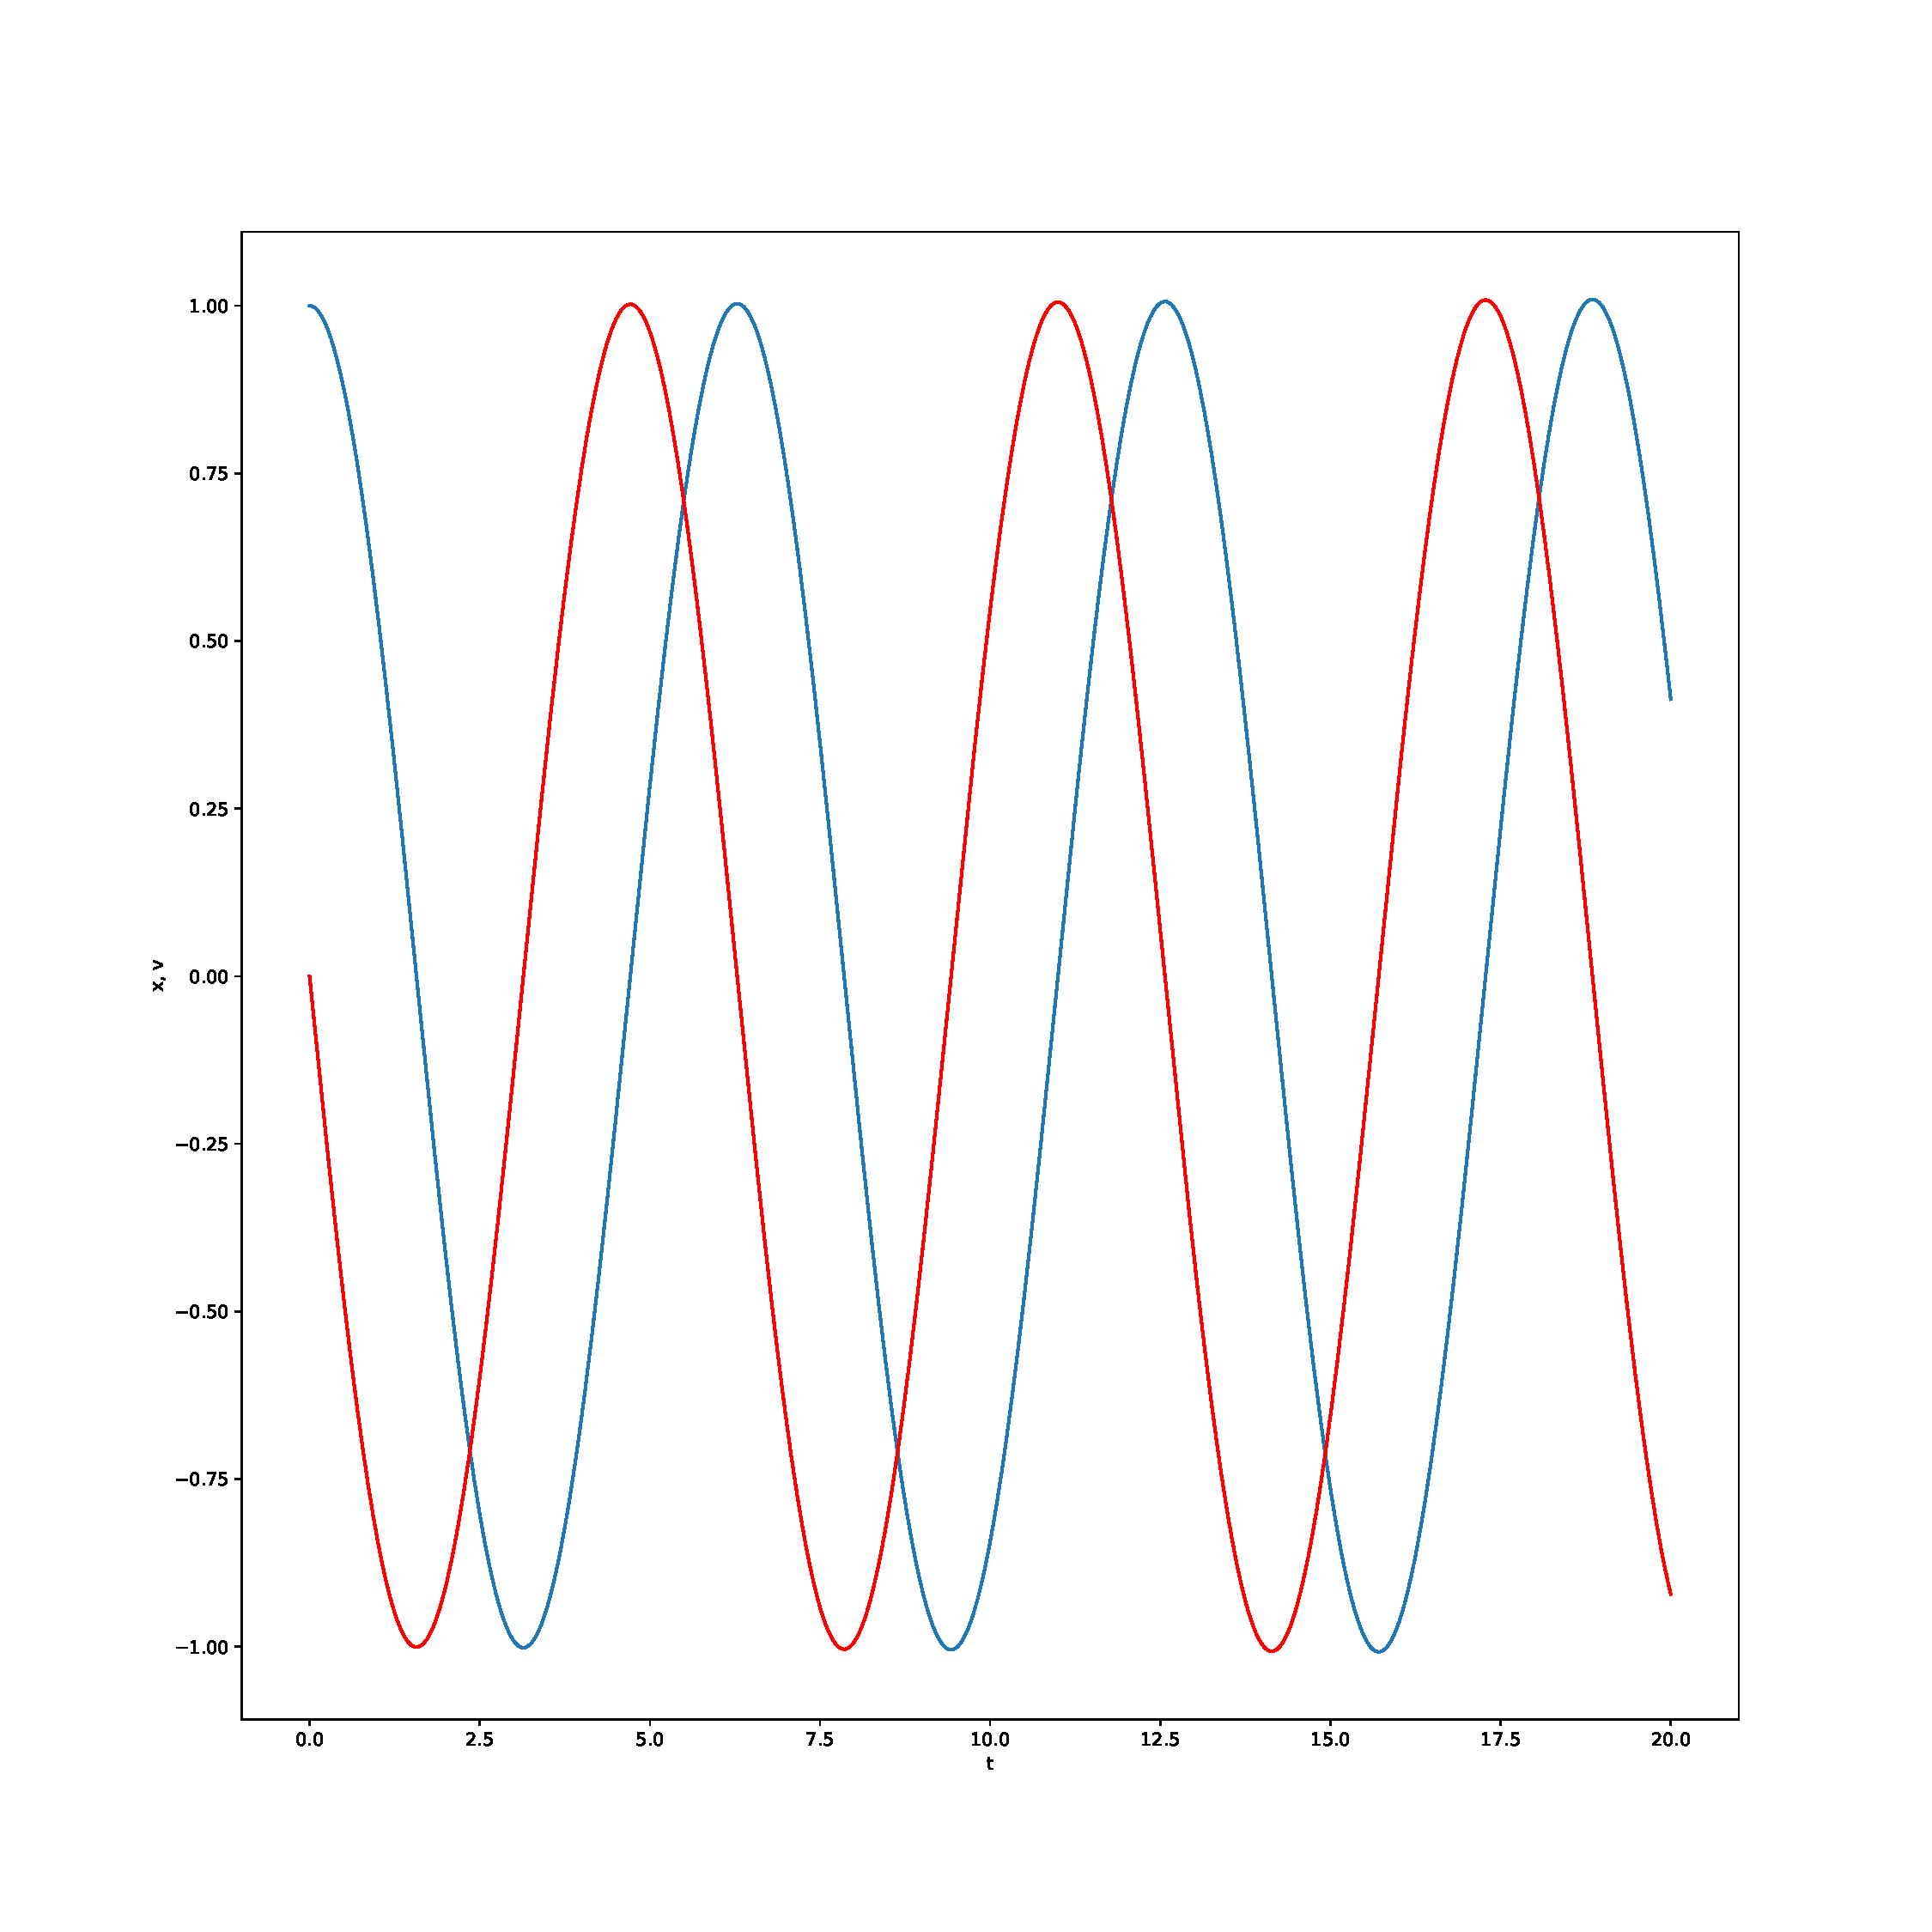
\includegraphics[width=.3\textwidth, height=.25\textheight]{explicitEuler.pdf}
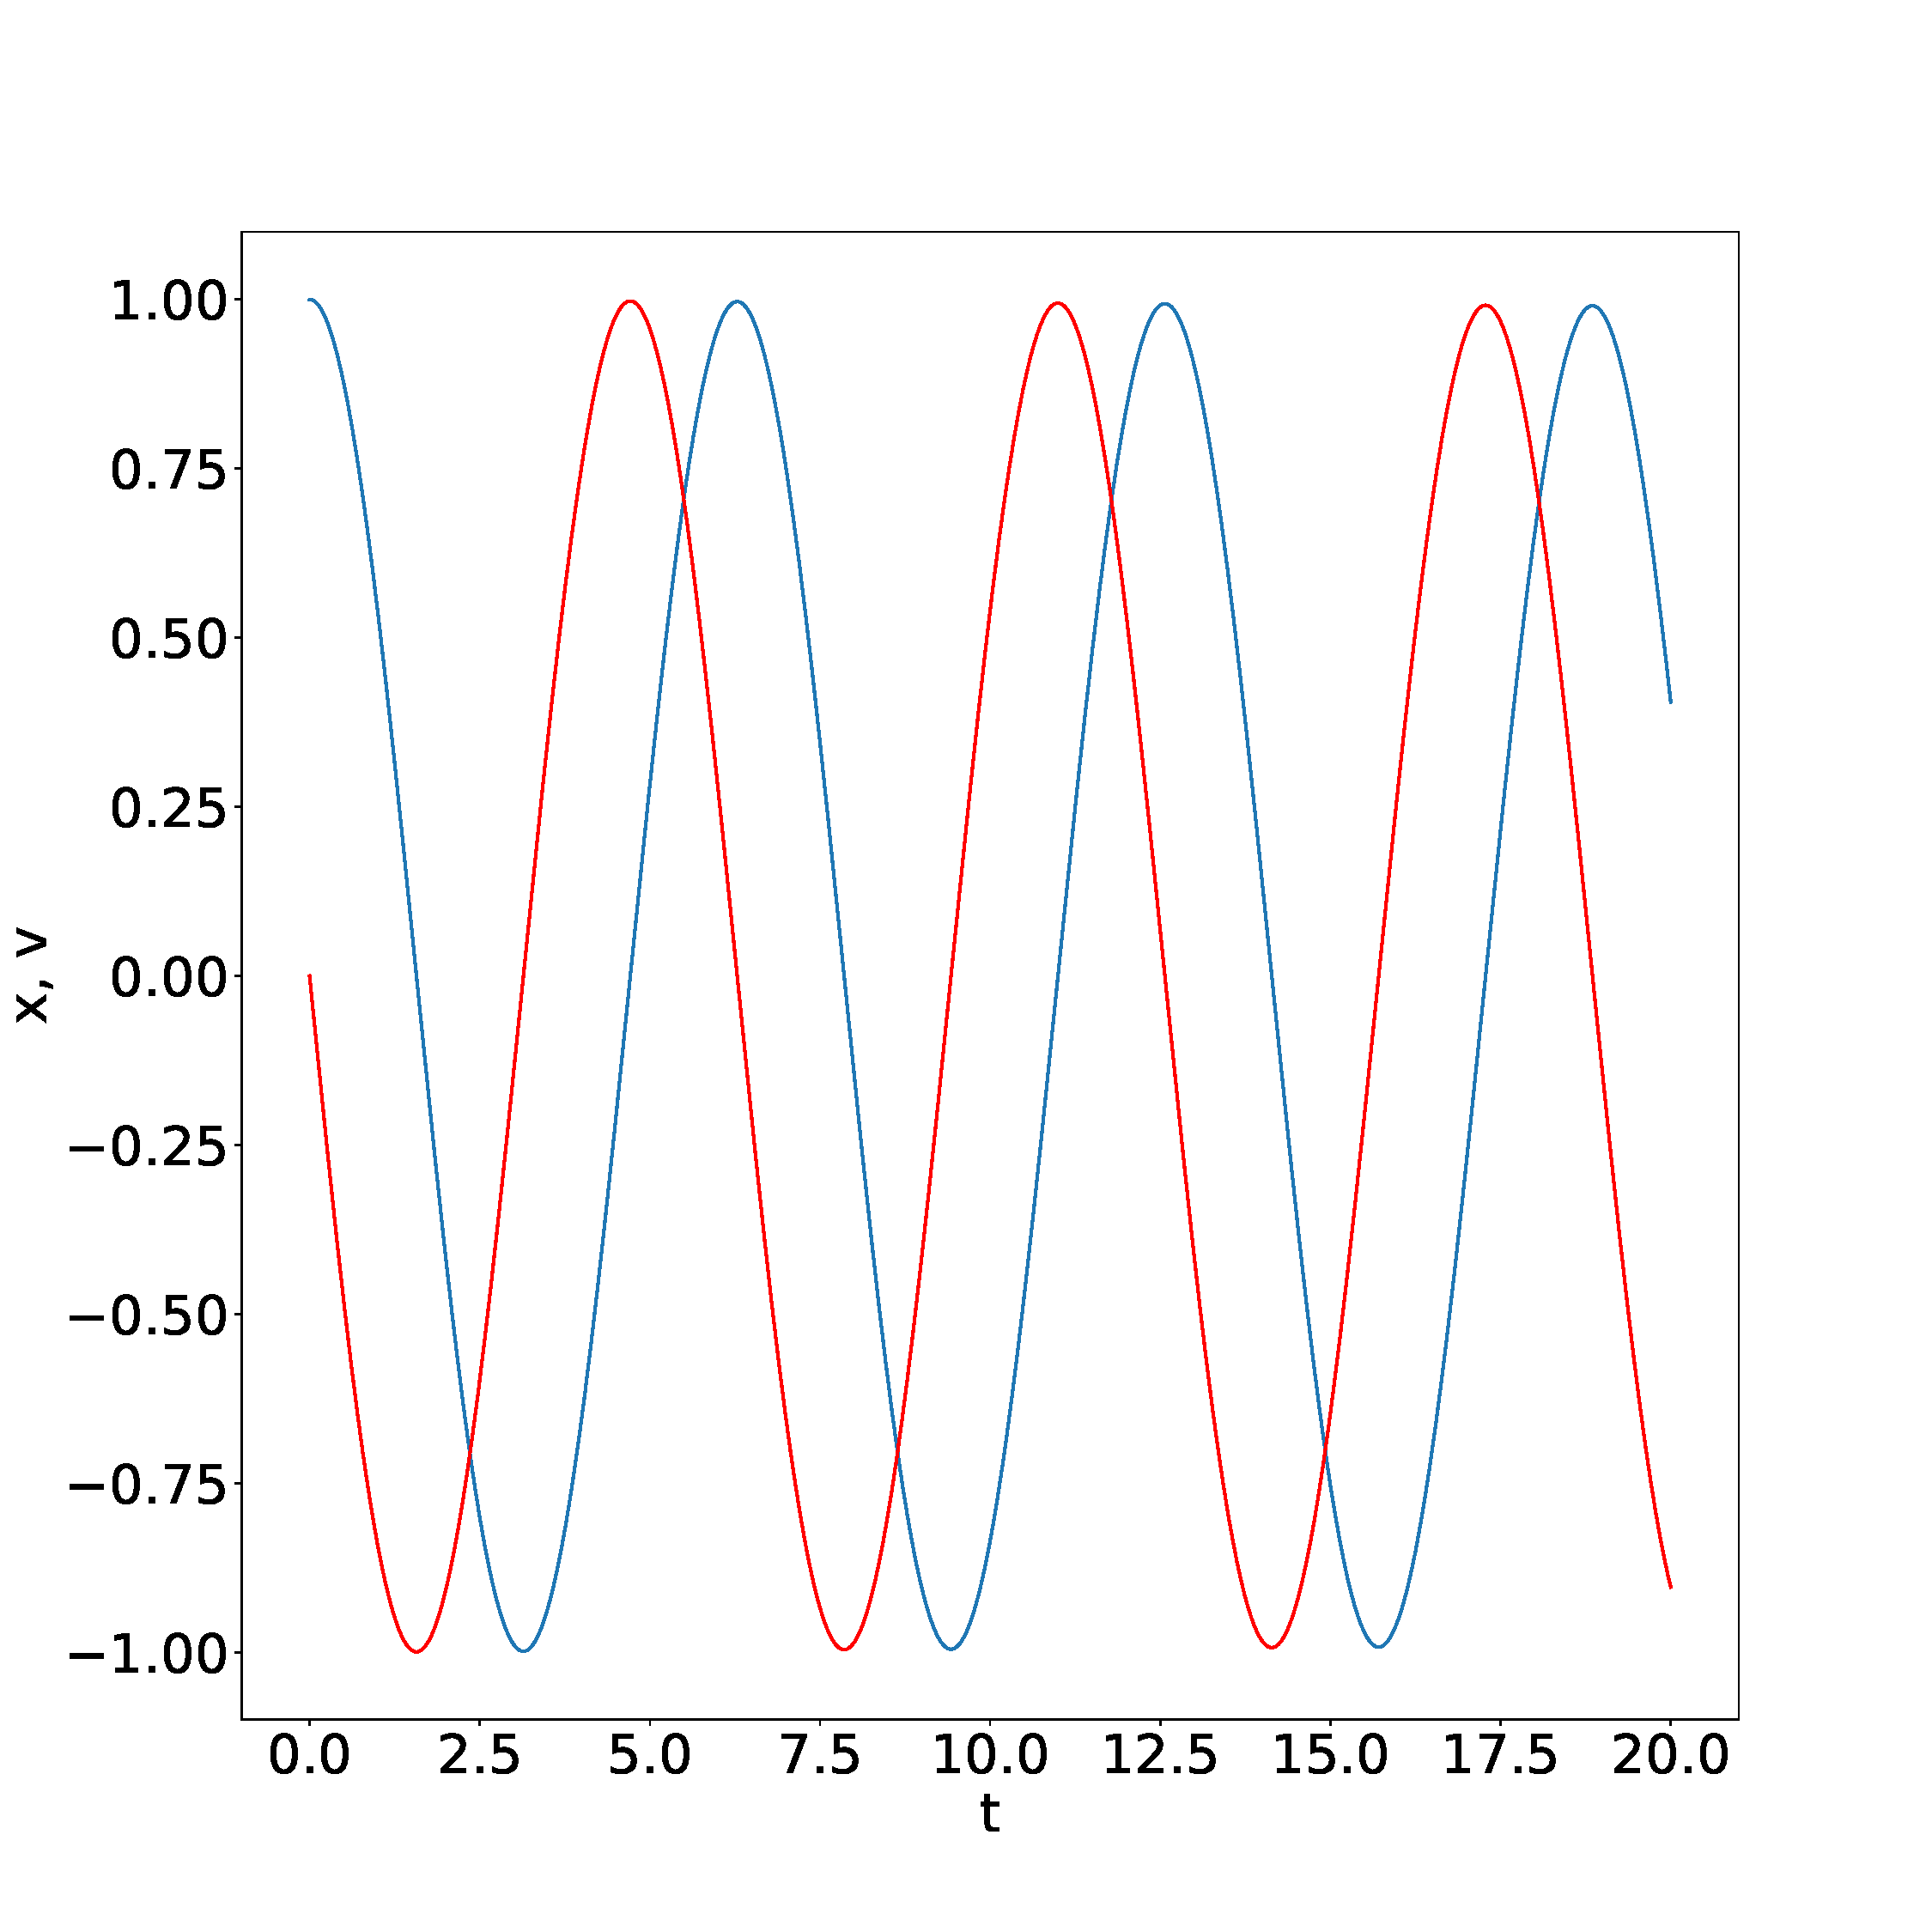
\includegraphics[width=.3\textwidth, height=.25\textheight]{implicitEuler.pdf}
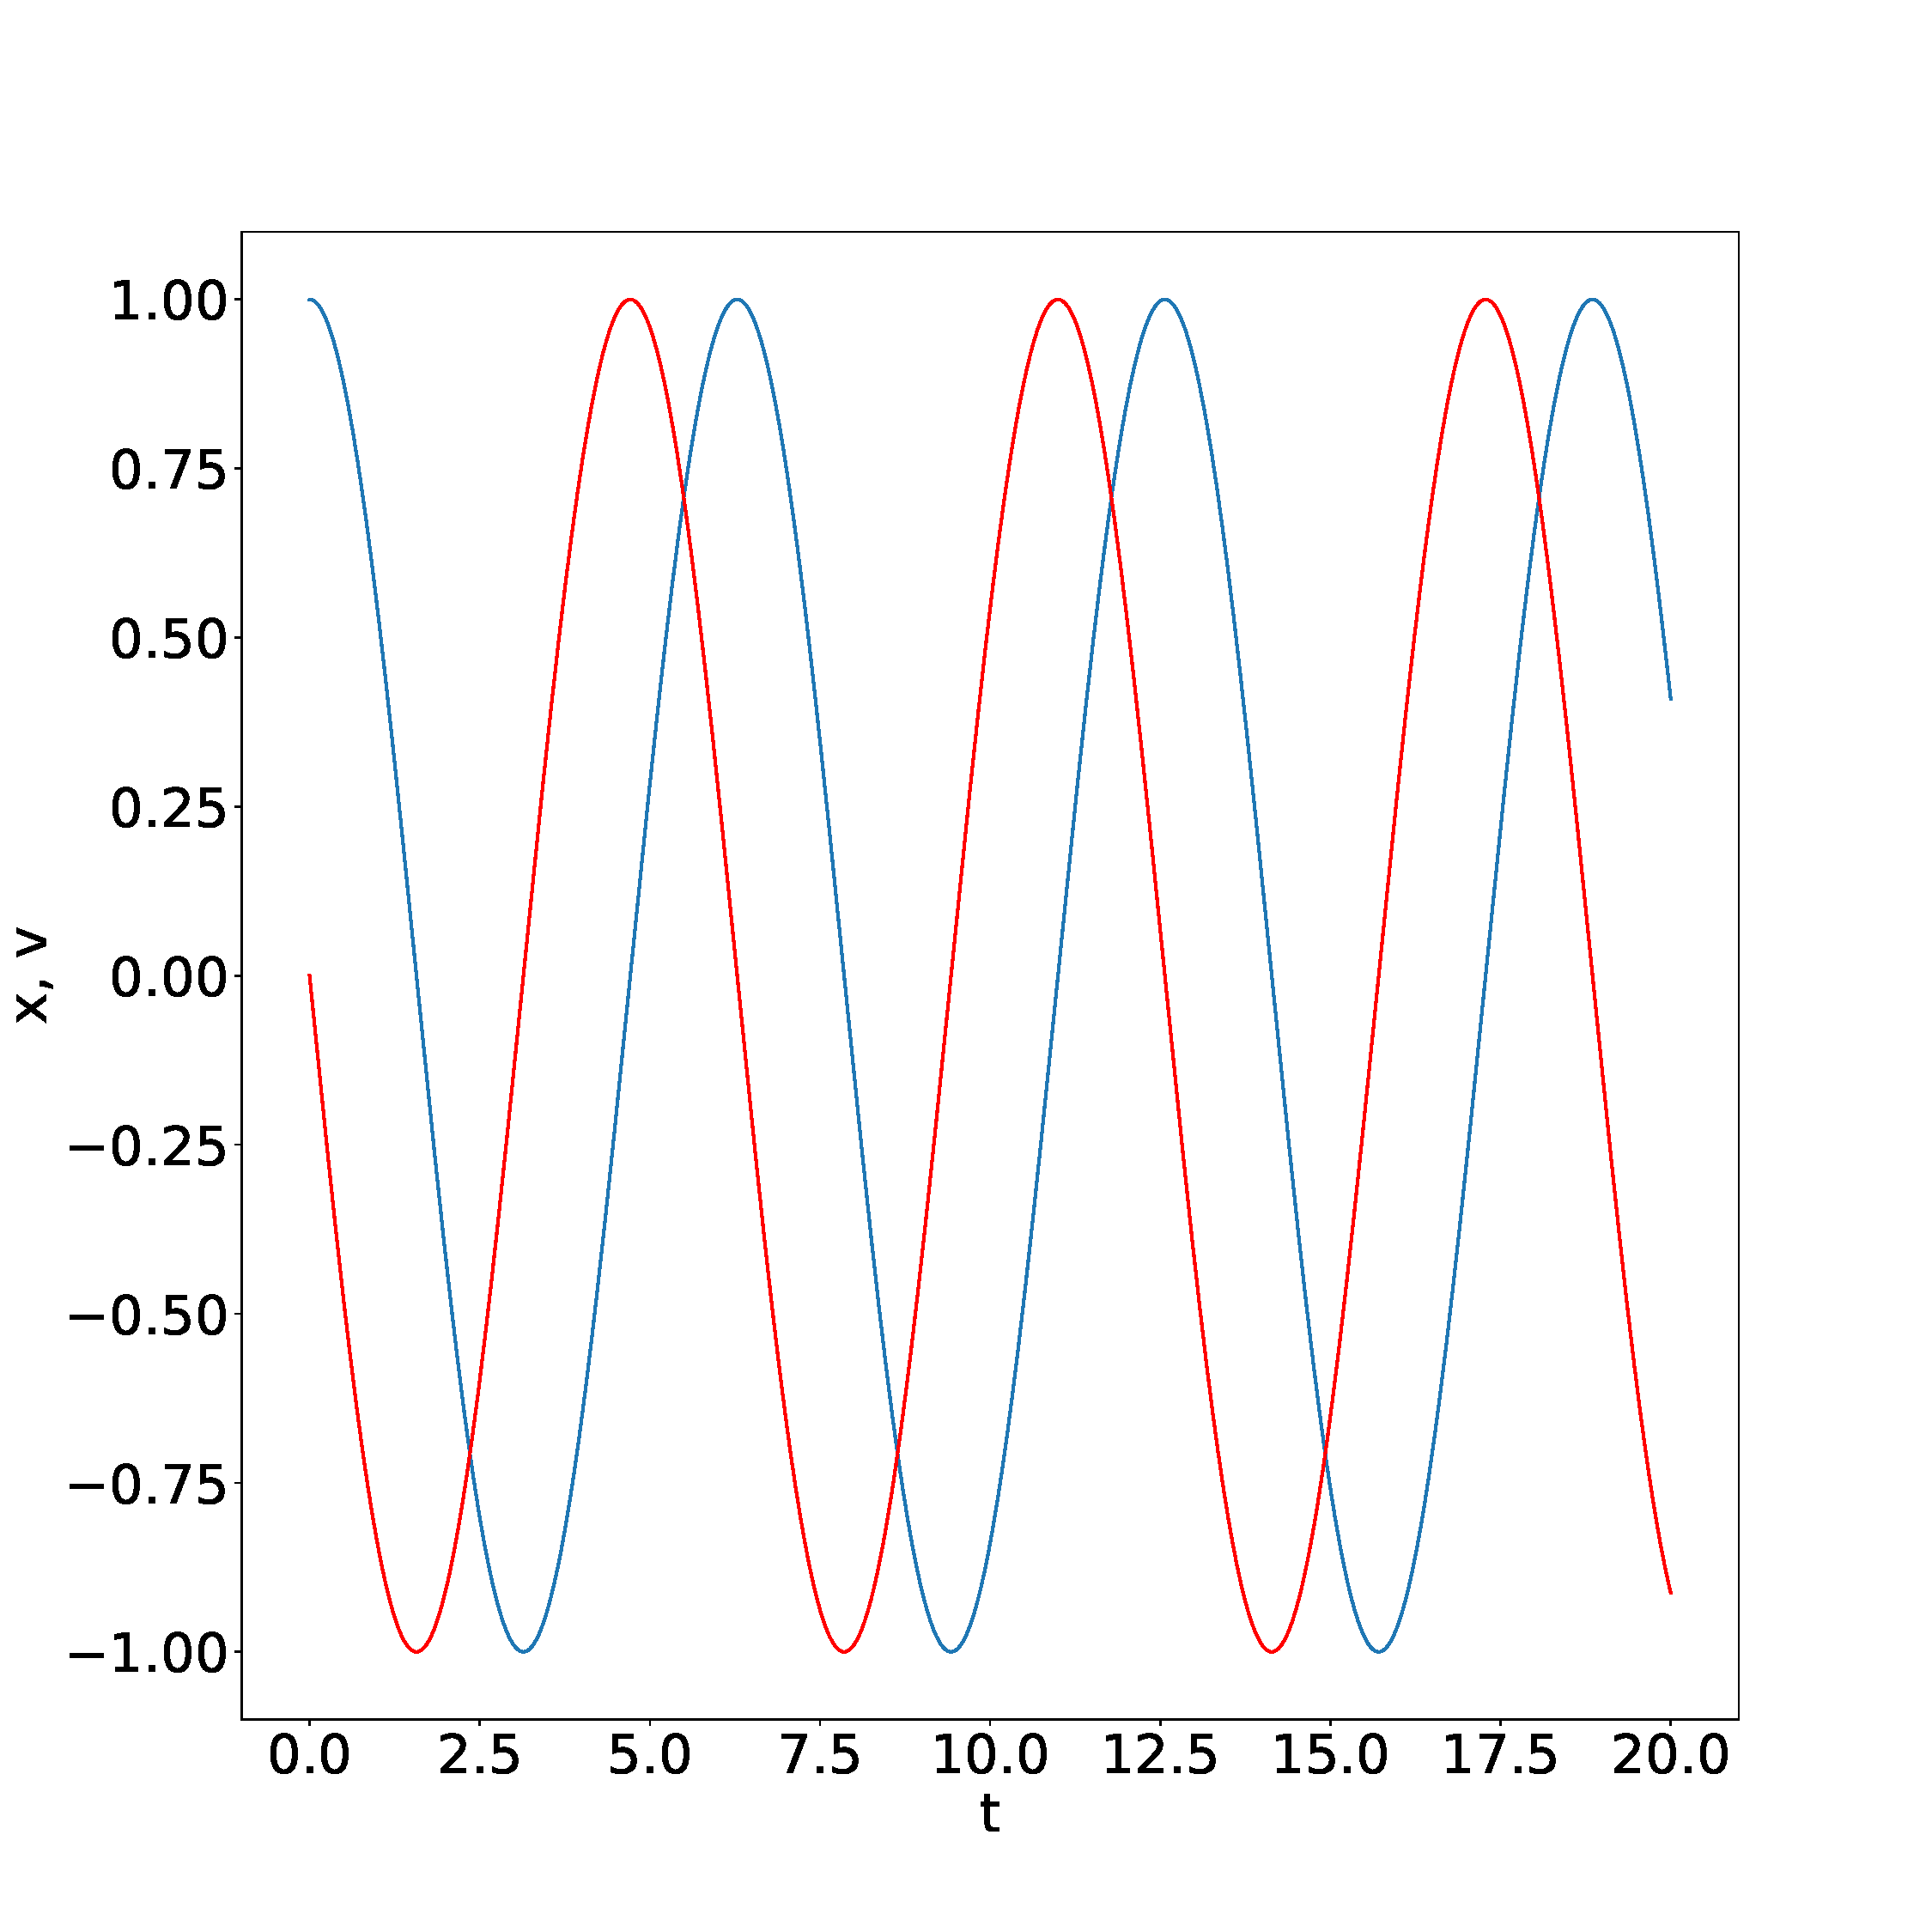
\includegraphics[width=.3\textwidth, height=.25\textheight]{trueState.pdf}
\caption{Plots of velocity (red) and displacement (blue) as a function of time for the explicit (left) and implicit (middle) Euler methods, compared to the exact solution (right). As we can see, both plots oscillate sinusoidally for velocity and displacement, and match the exact solution almost identically. All plots are made with $x(0) = 1$, $v(0) = 0$, $t(0) = 0$, and $h = .001$.}
\end{figure}

\begin{figure}[H]
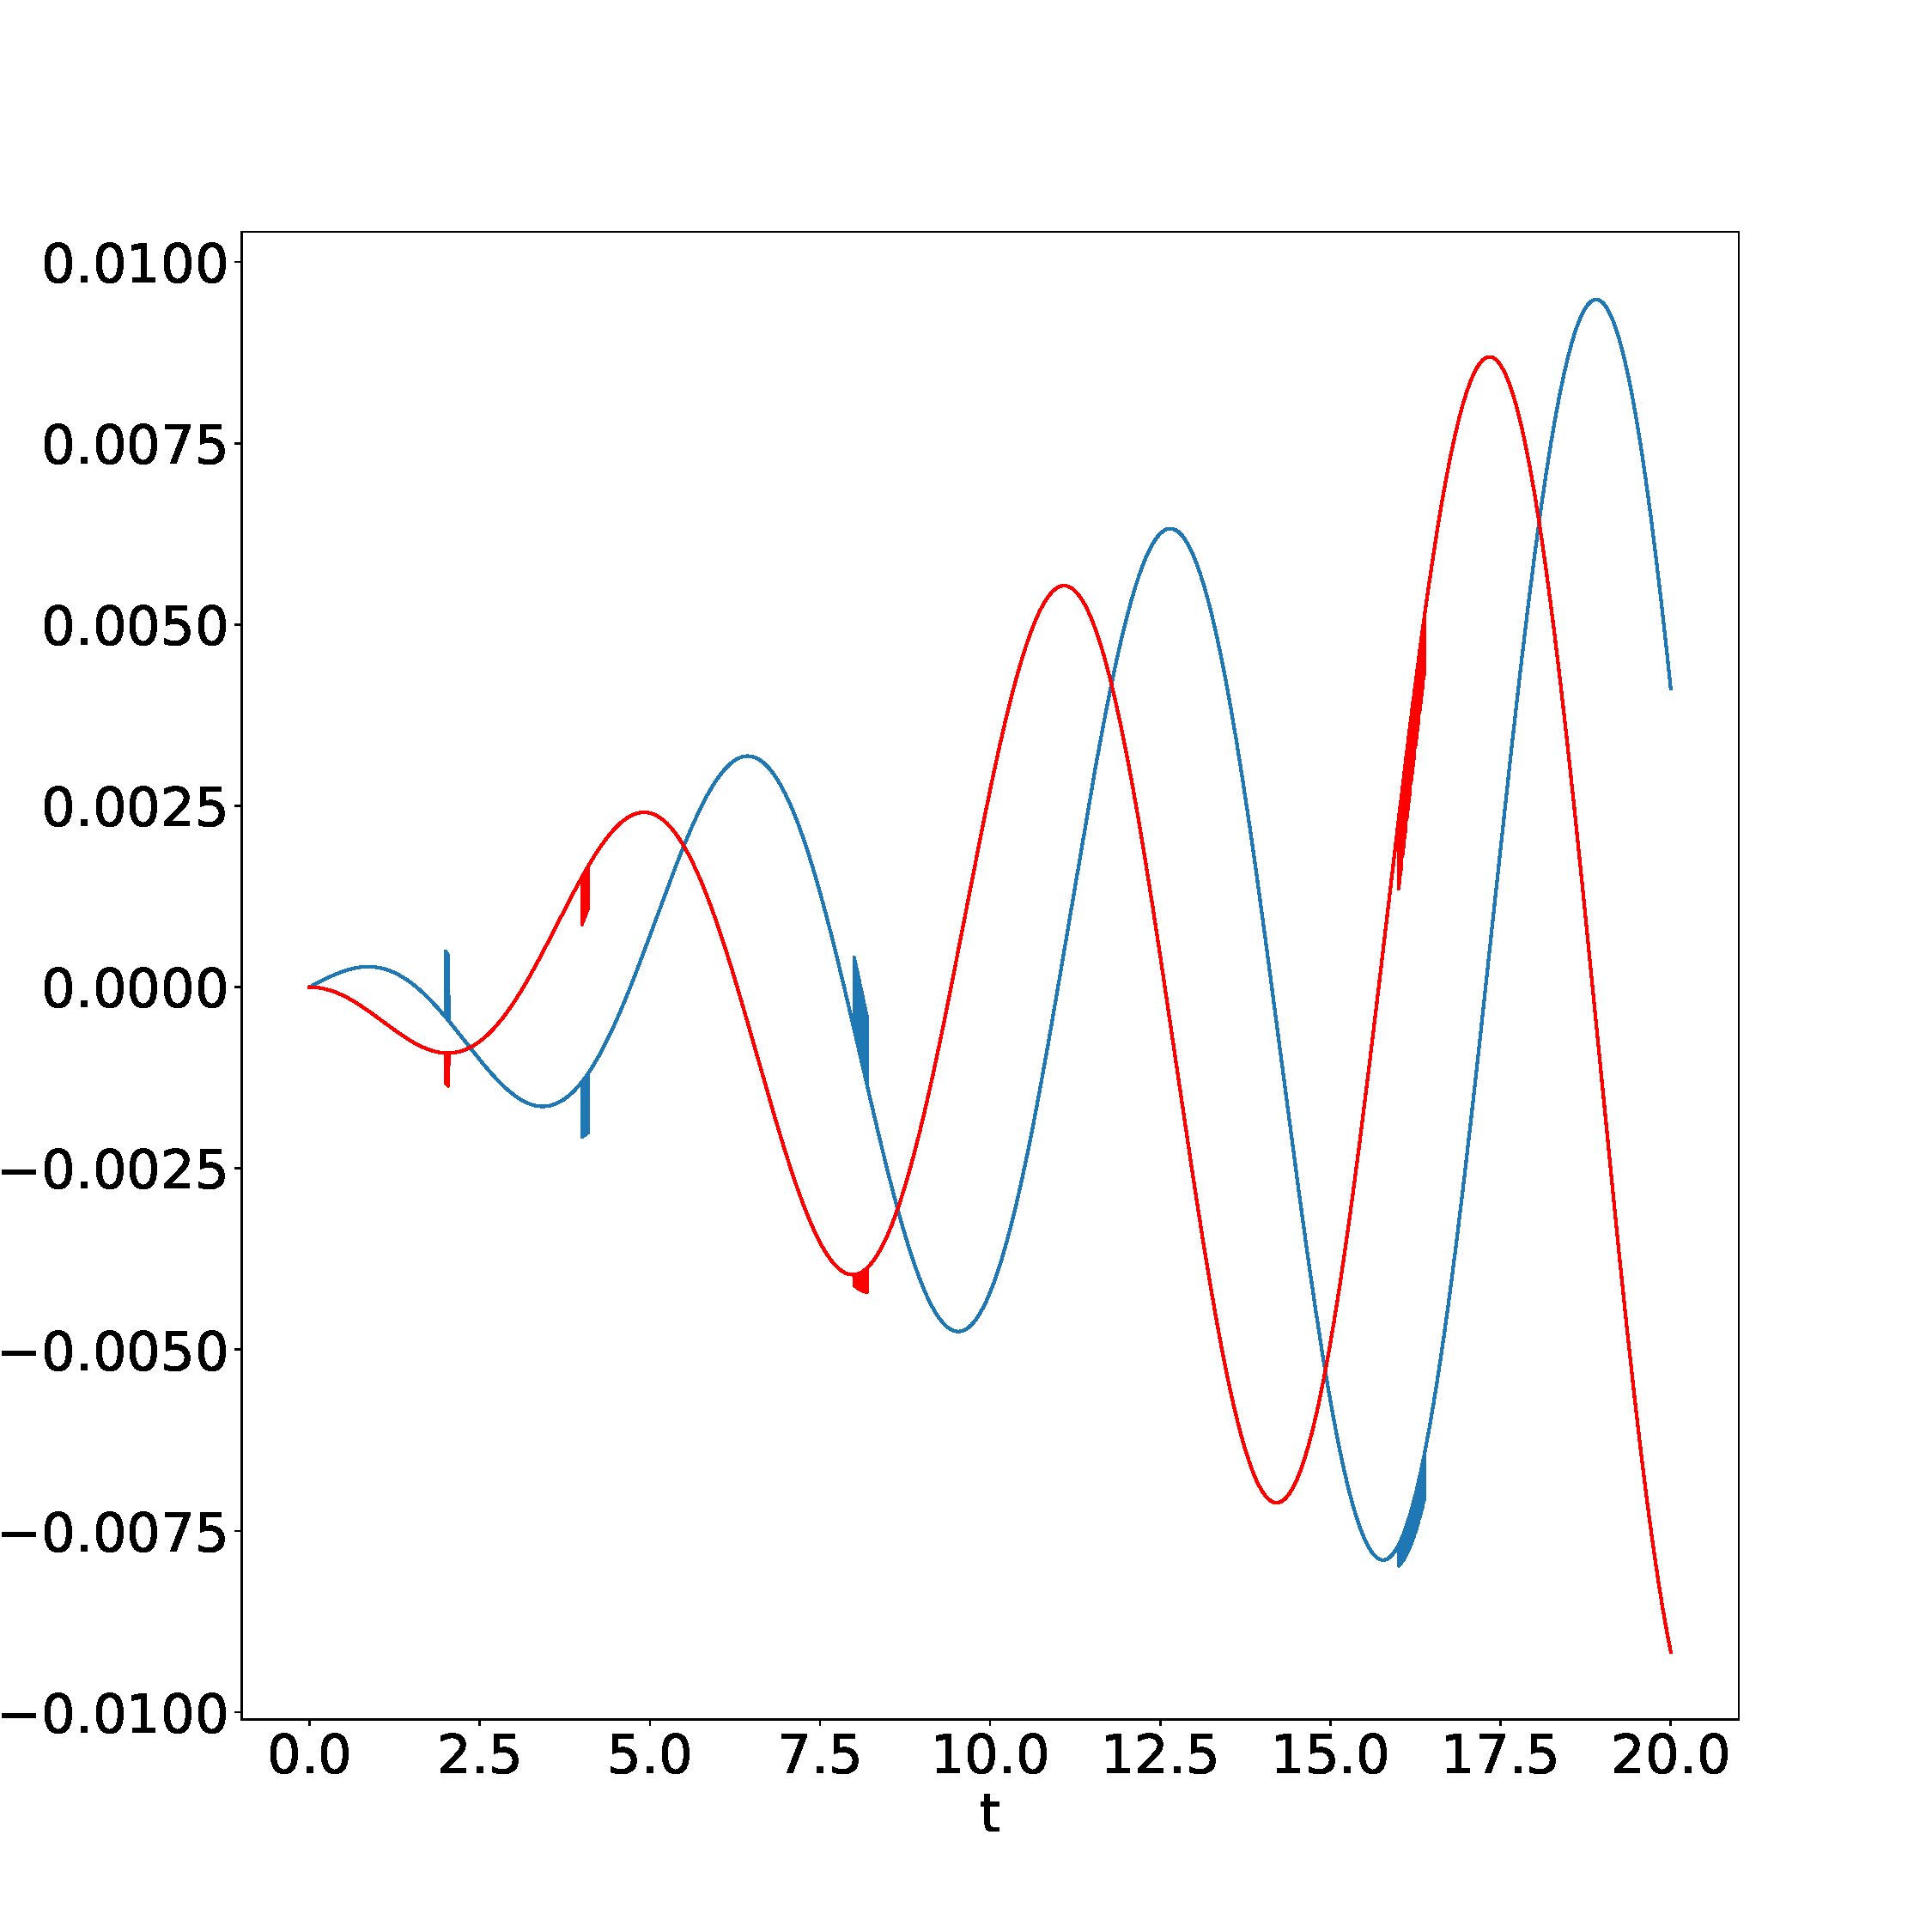
\includegraphics[width=.5\textwidth, height=.35\textheight]{errorPlot1.pdf}
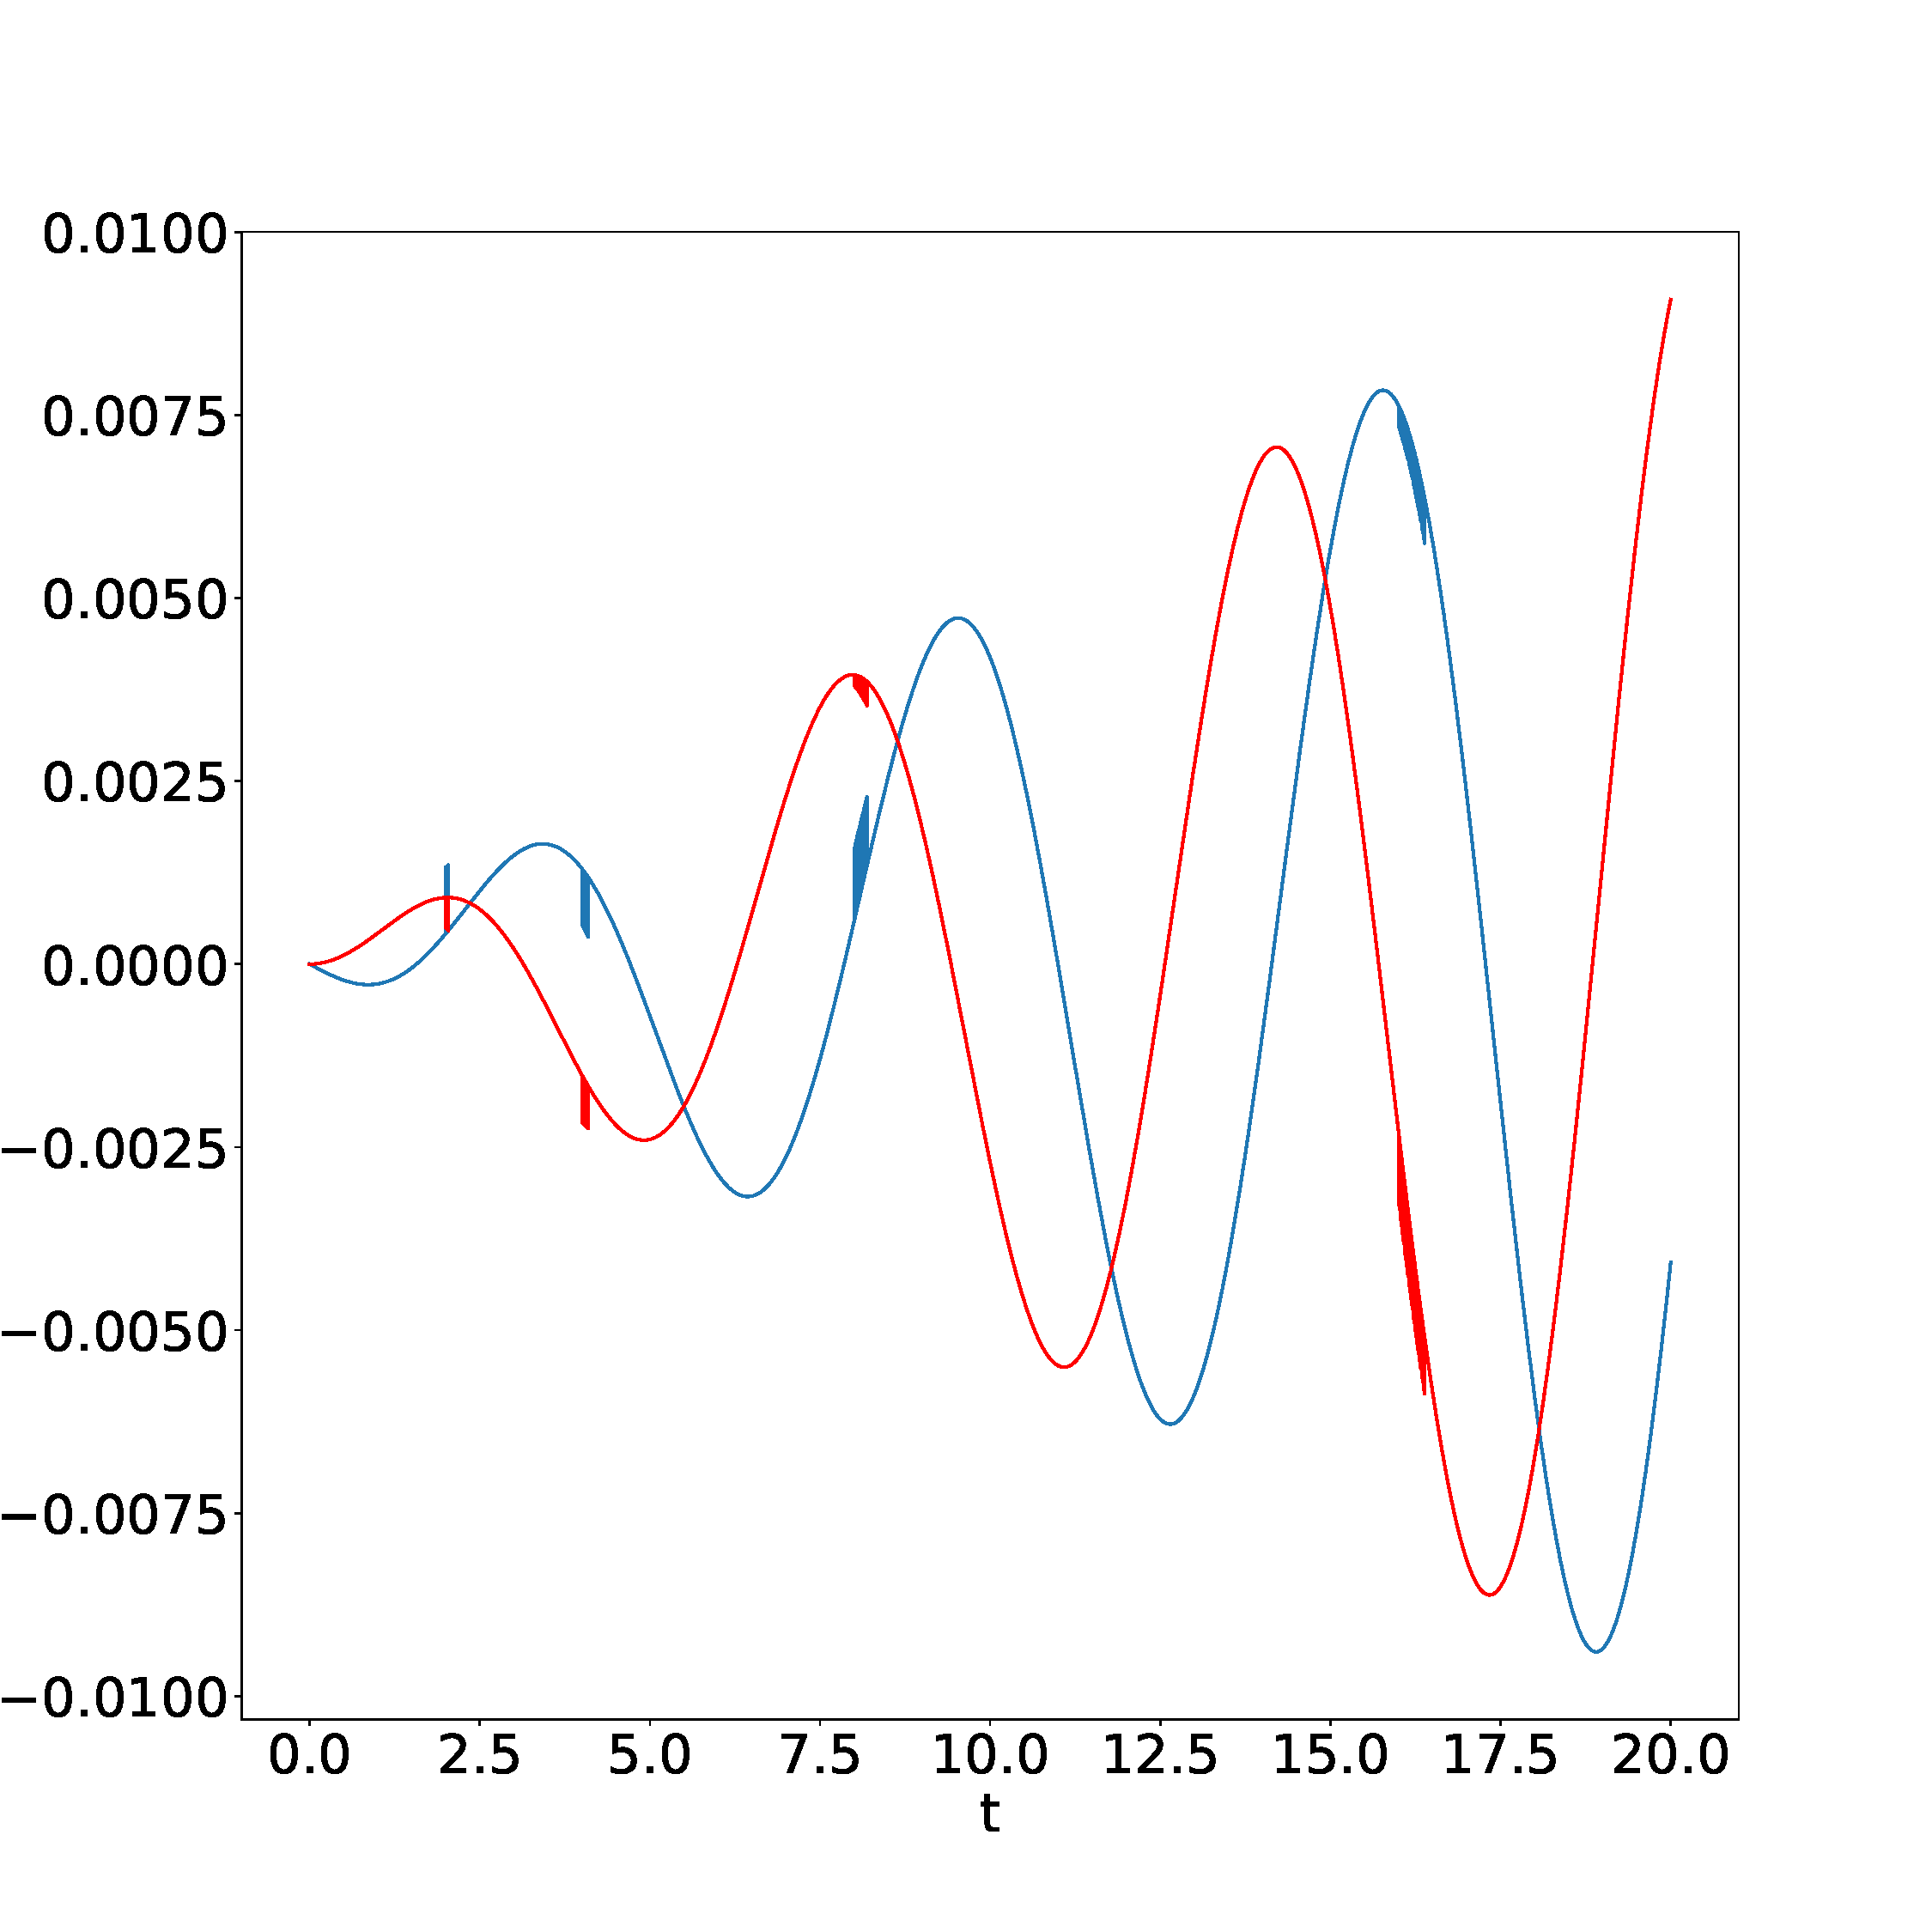
\includegraphics[width=.5\textwidth, height=.35\textheight]{errorPlot2.pdf}
\caption{Plots of velocity error (red) and displacement error (blue) as a function of time for the explicit (left) and implicit (right) Euler methods, with respect to the exact solution. The error of both the explicit and implicit methods grows with time, and oscillates sinusoidally. Both plots are made with $x(0) = 1$, $v(0) = 0$, $t(0) = 0$, and $h = .001$.}
\end{figure}

\begin{figure}[H]
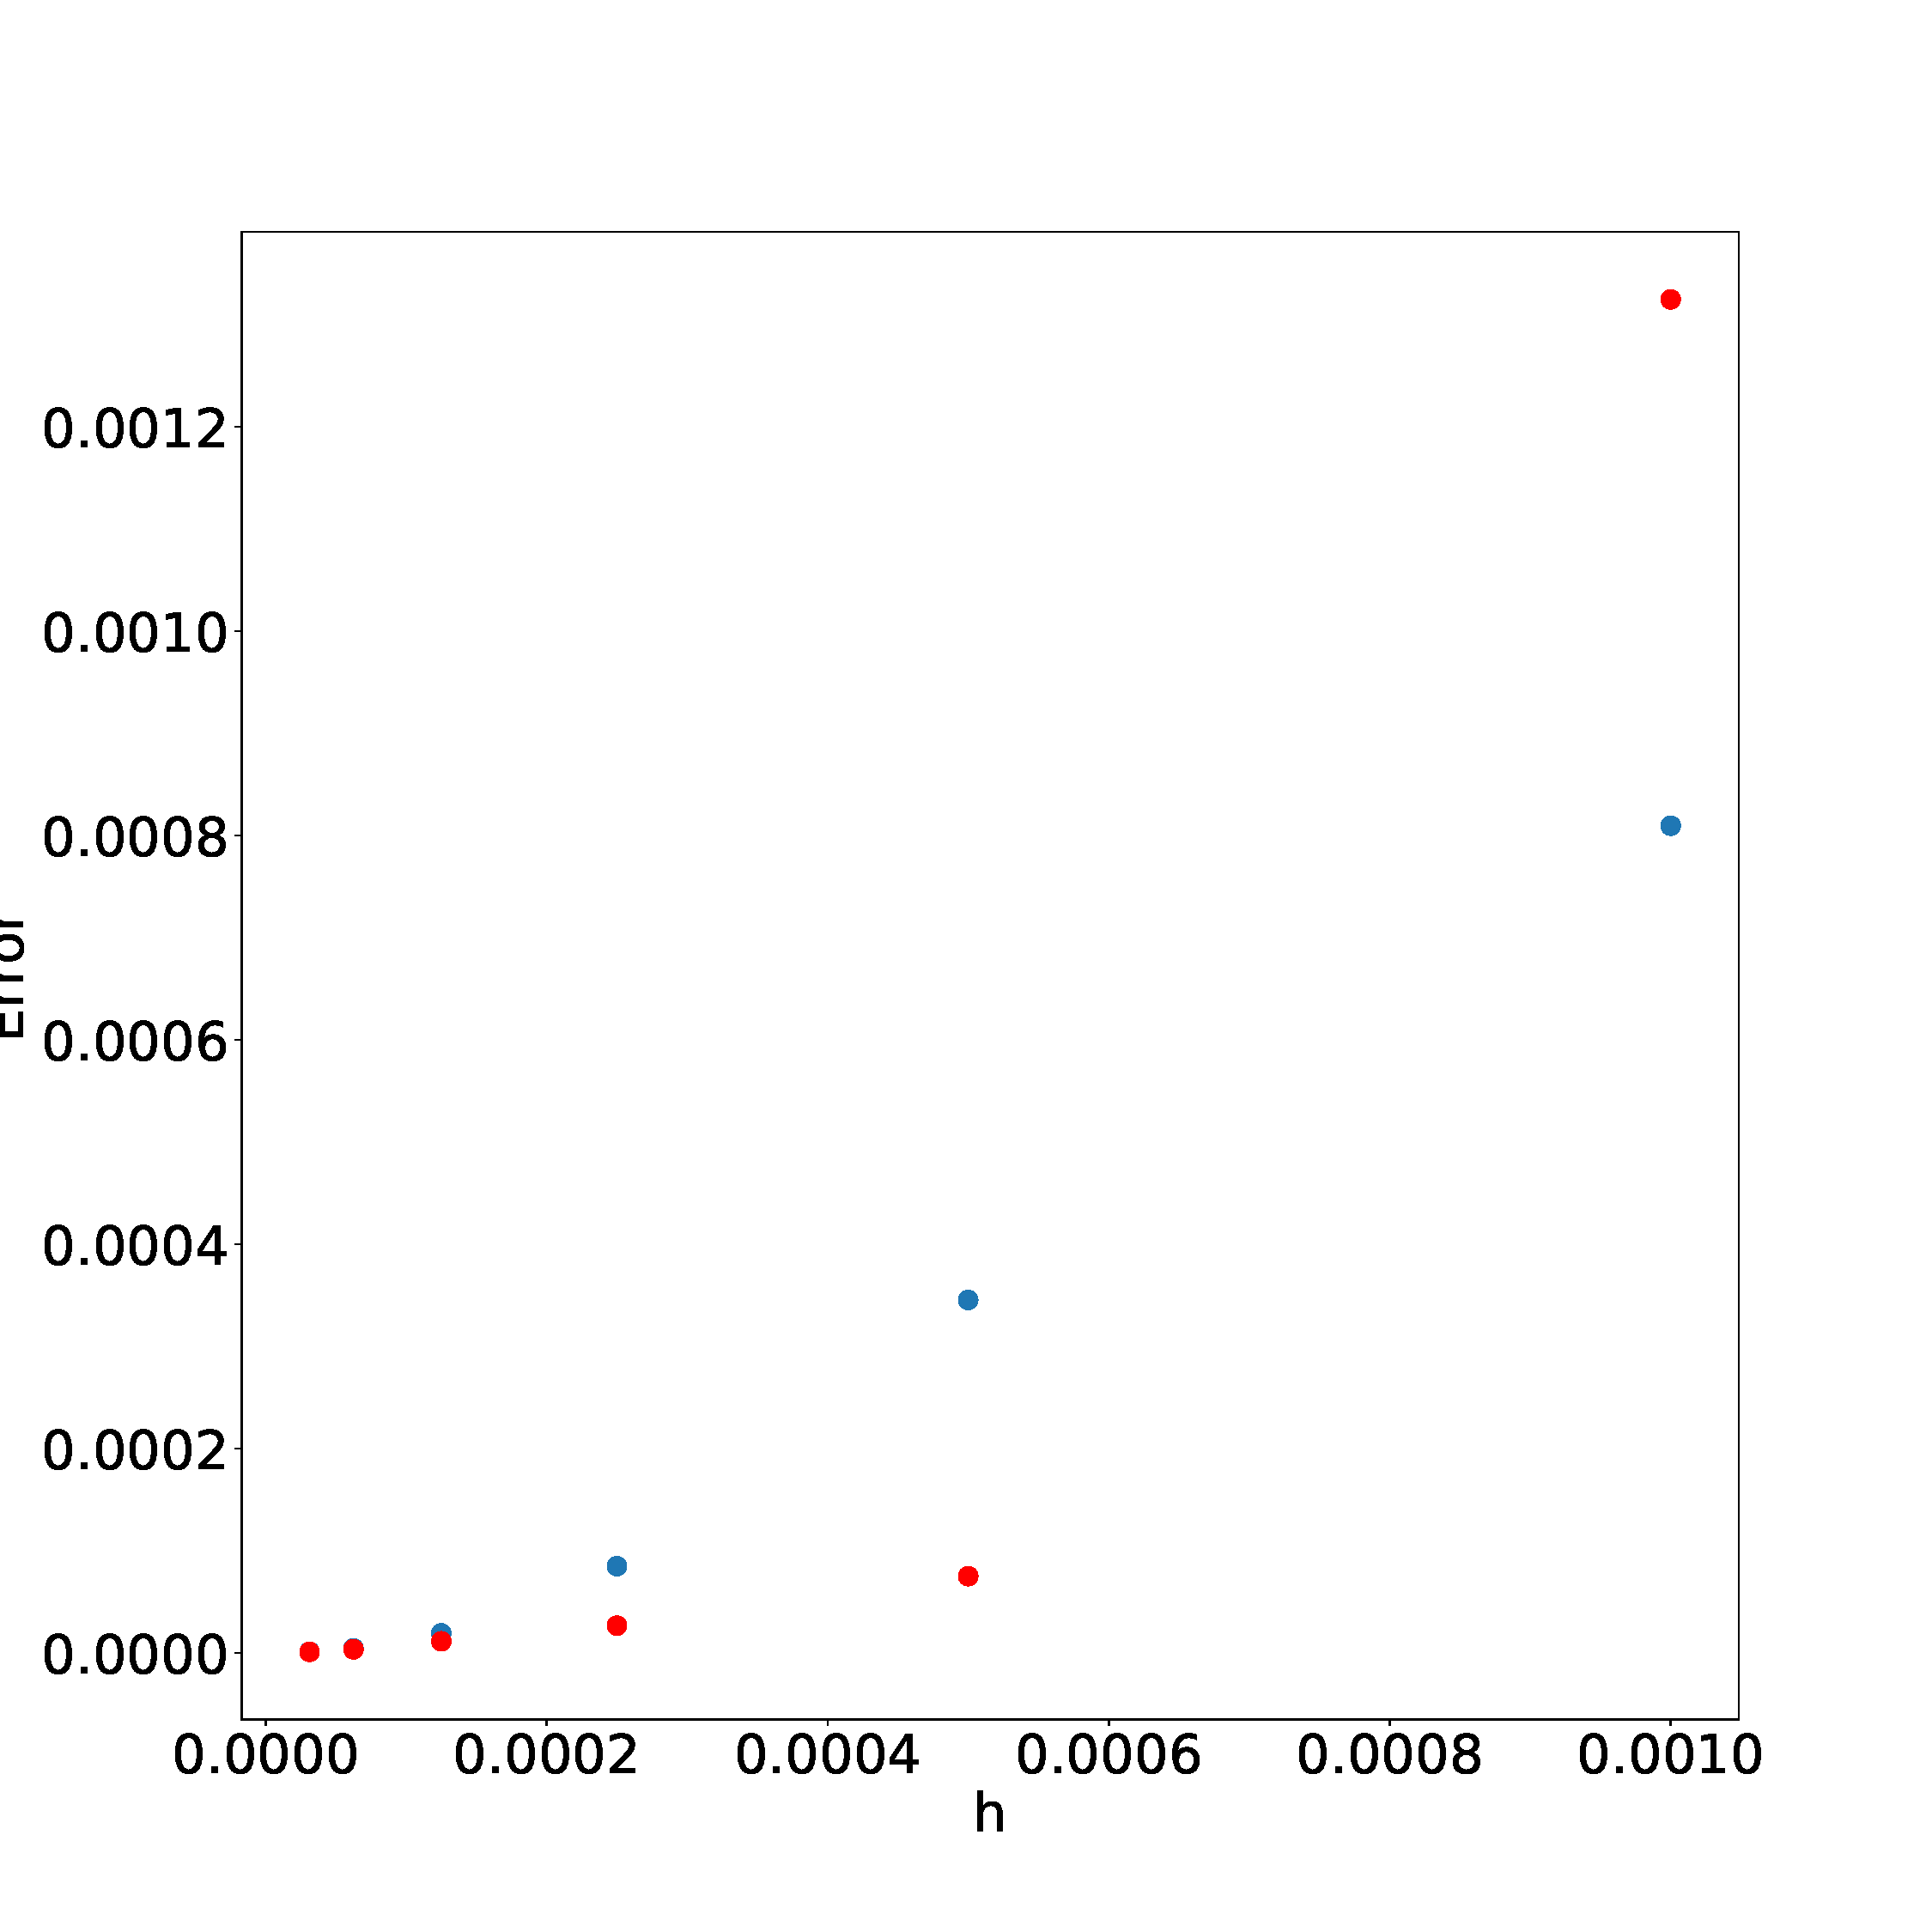
\includegraphics[width=.5\textwidth, height=.35\textheight]{errorvsH.pdf}
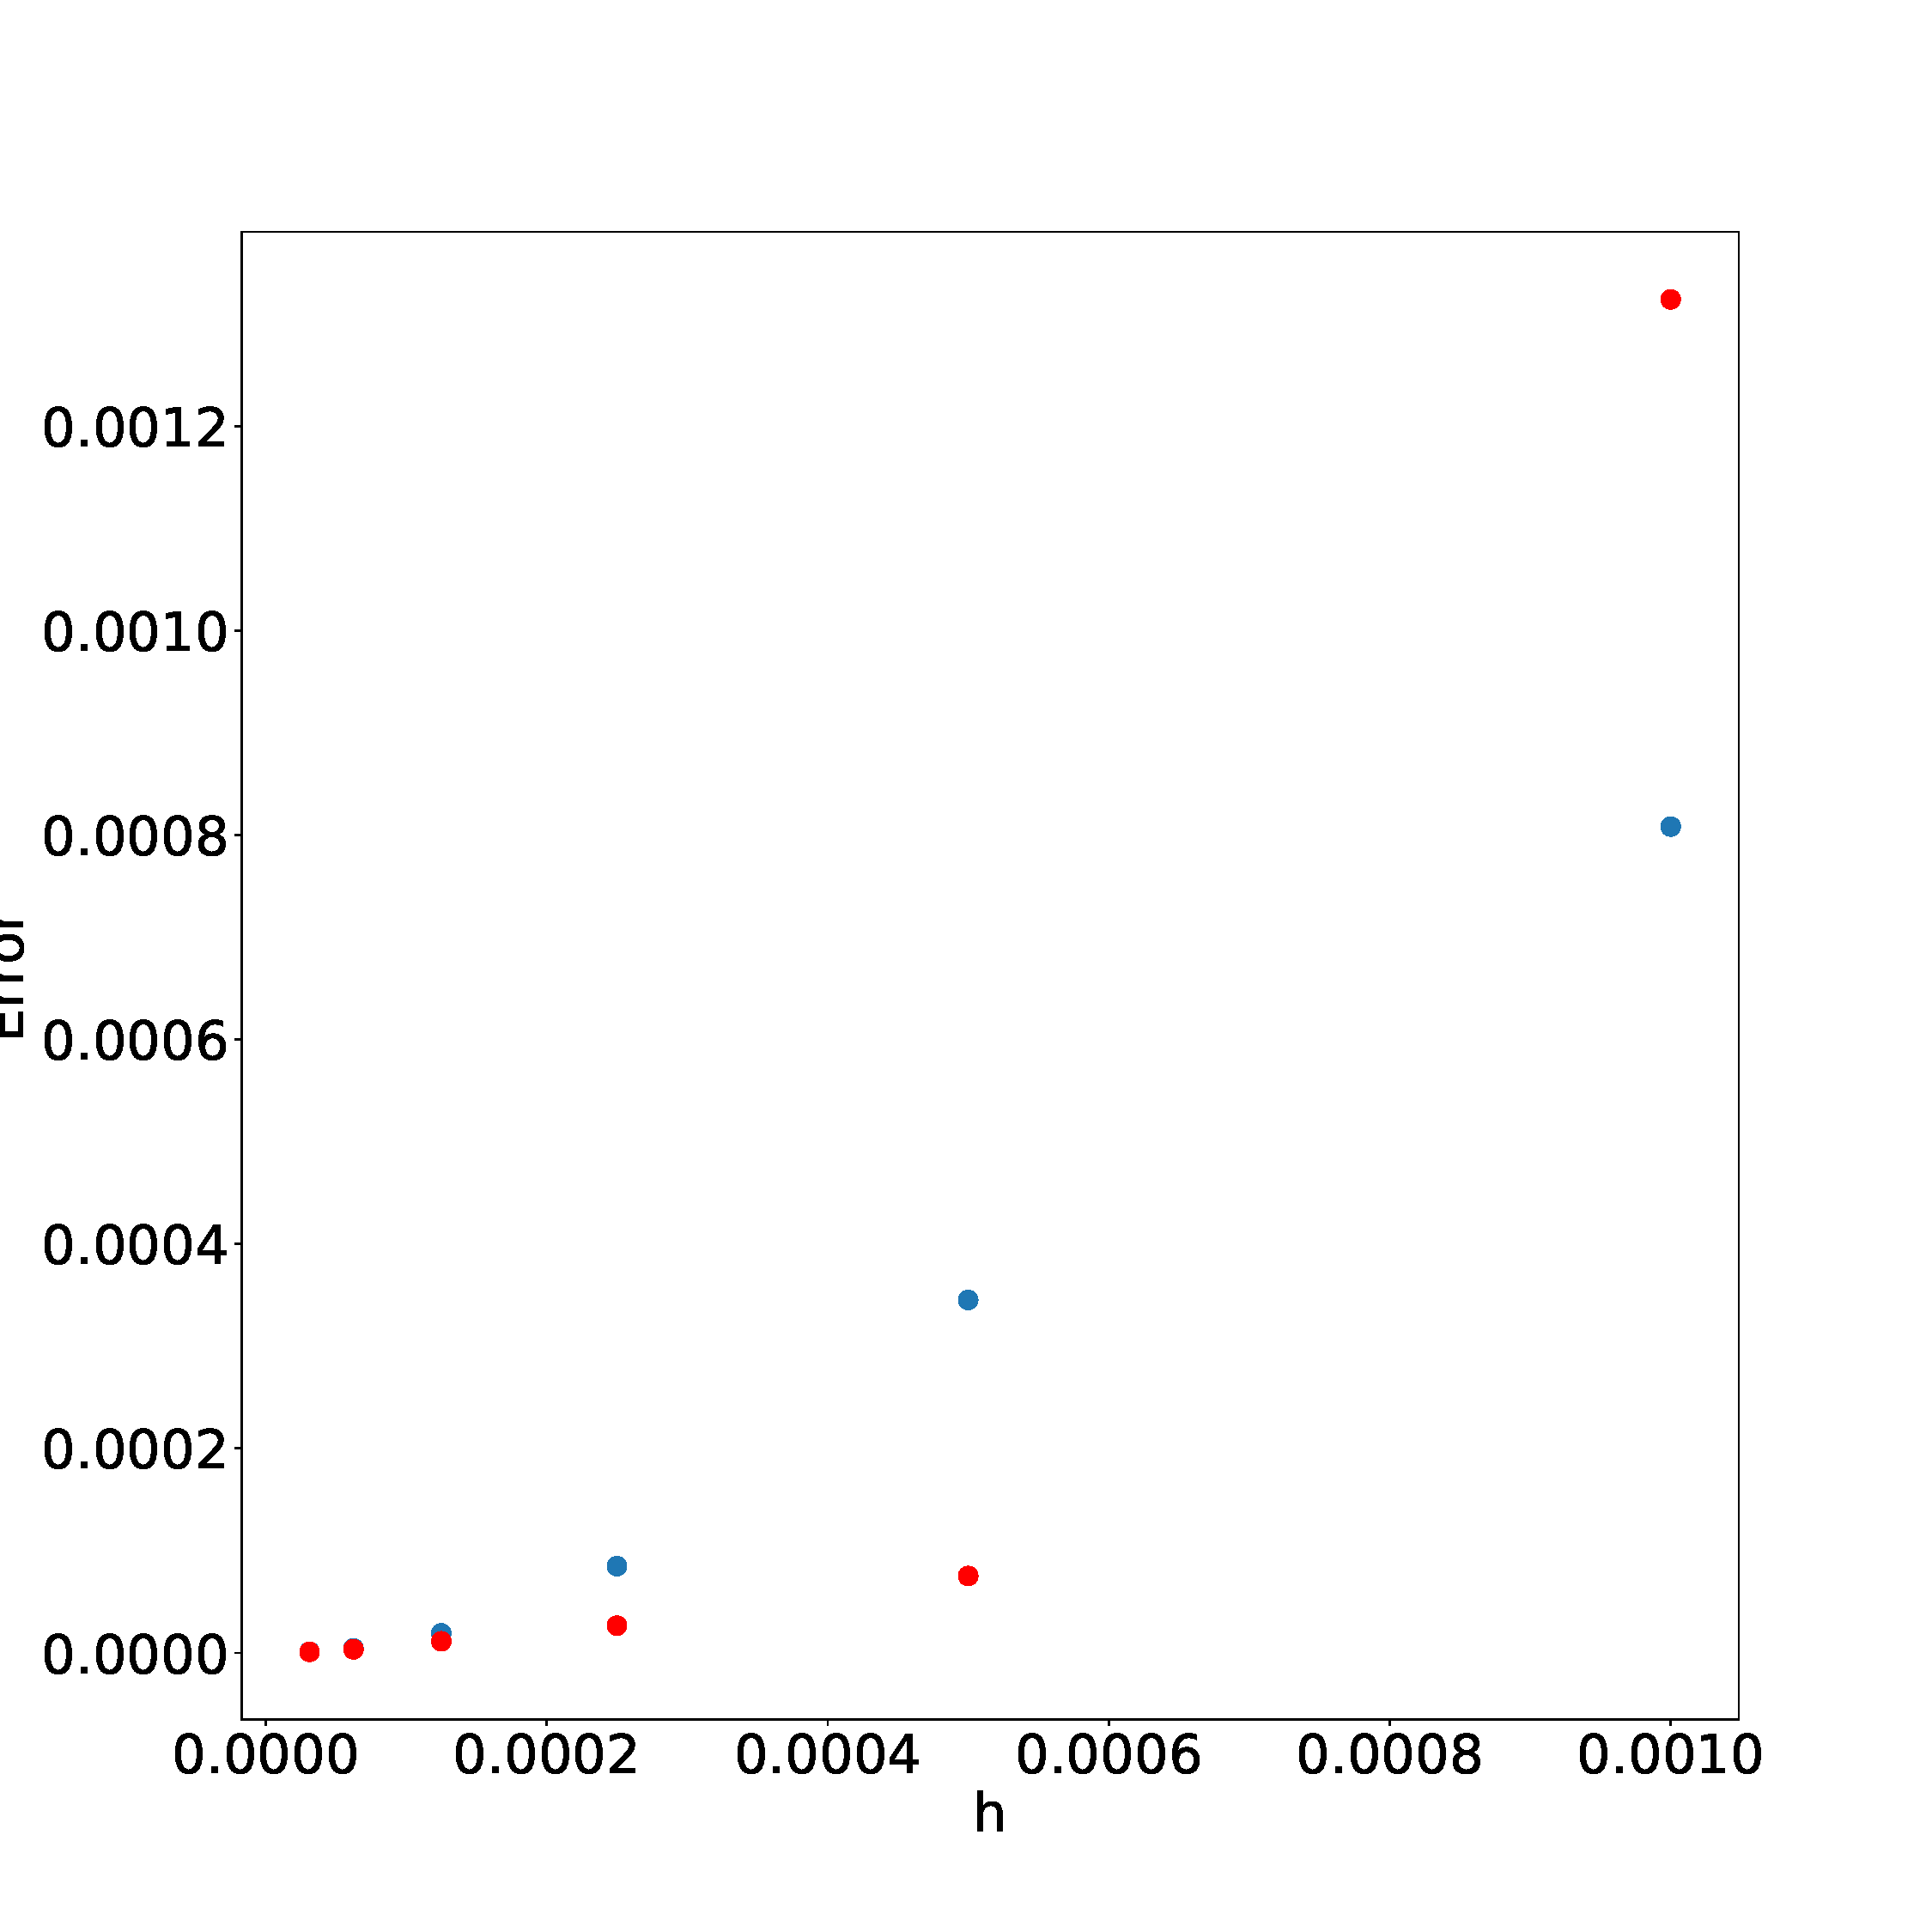
\includegraphics[width=.5\textwidth, height=.35\textheight]{errorvsH2.pdf}
\caption{Plots of maximum velocity error (red) and maximum displacement error (blue) with respect to the exact solution over several cycles at a given $h$ for the explicit (left) and implicit (right) Euler methods. The error of velocity and position respect linear relationships for sufficiently small $h$. Both plots are made with $x(0) = 1$, $v(0) = 1$, and $t(0) = 0$.}
\end{figure}

\begin{figure}[H]
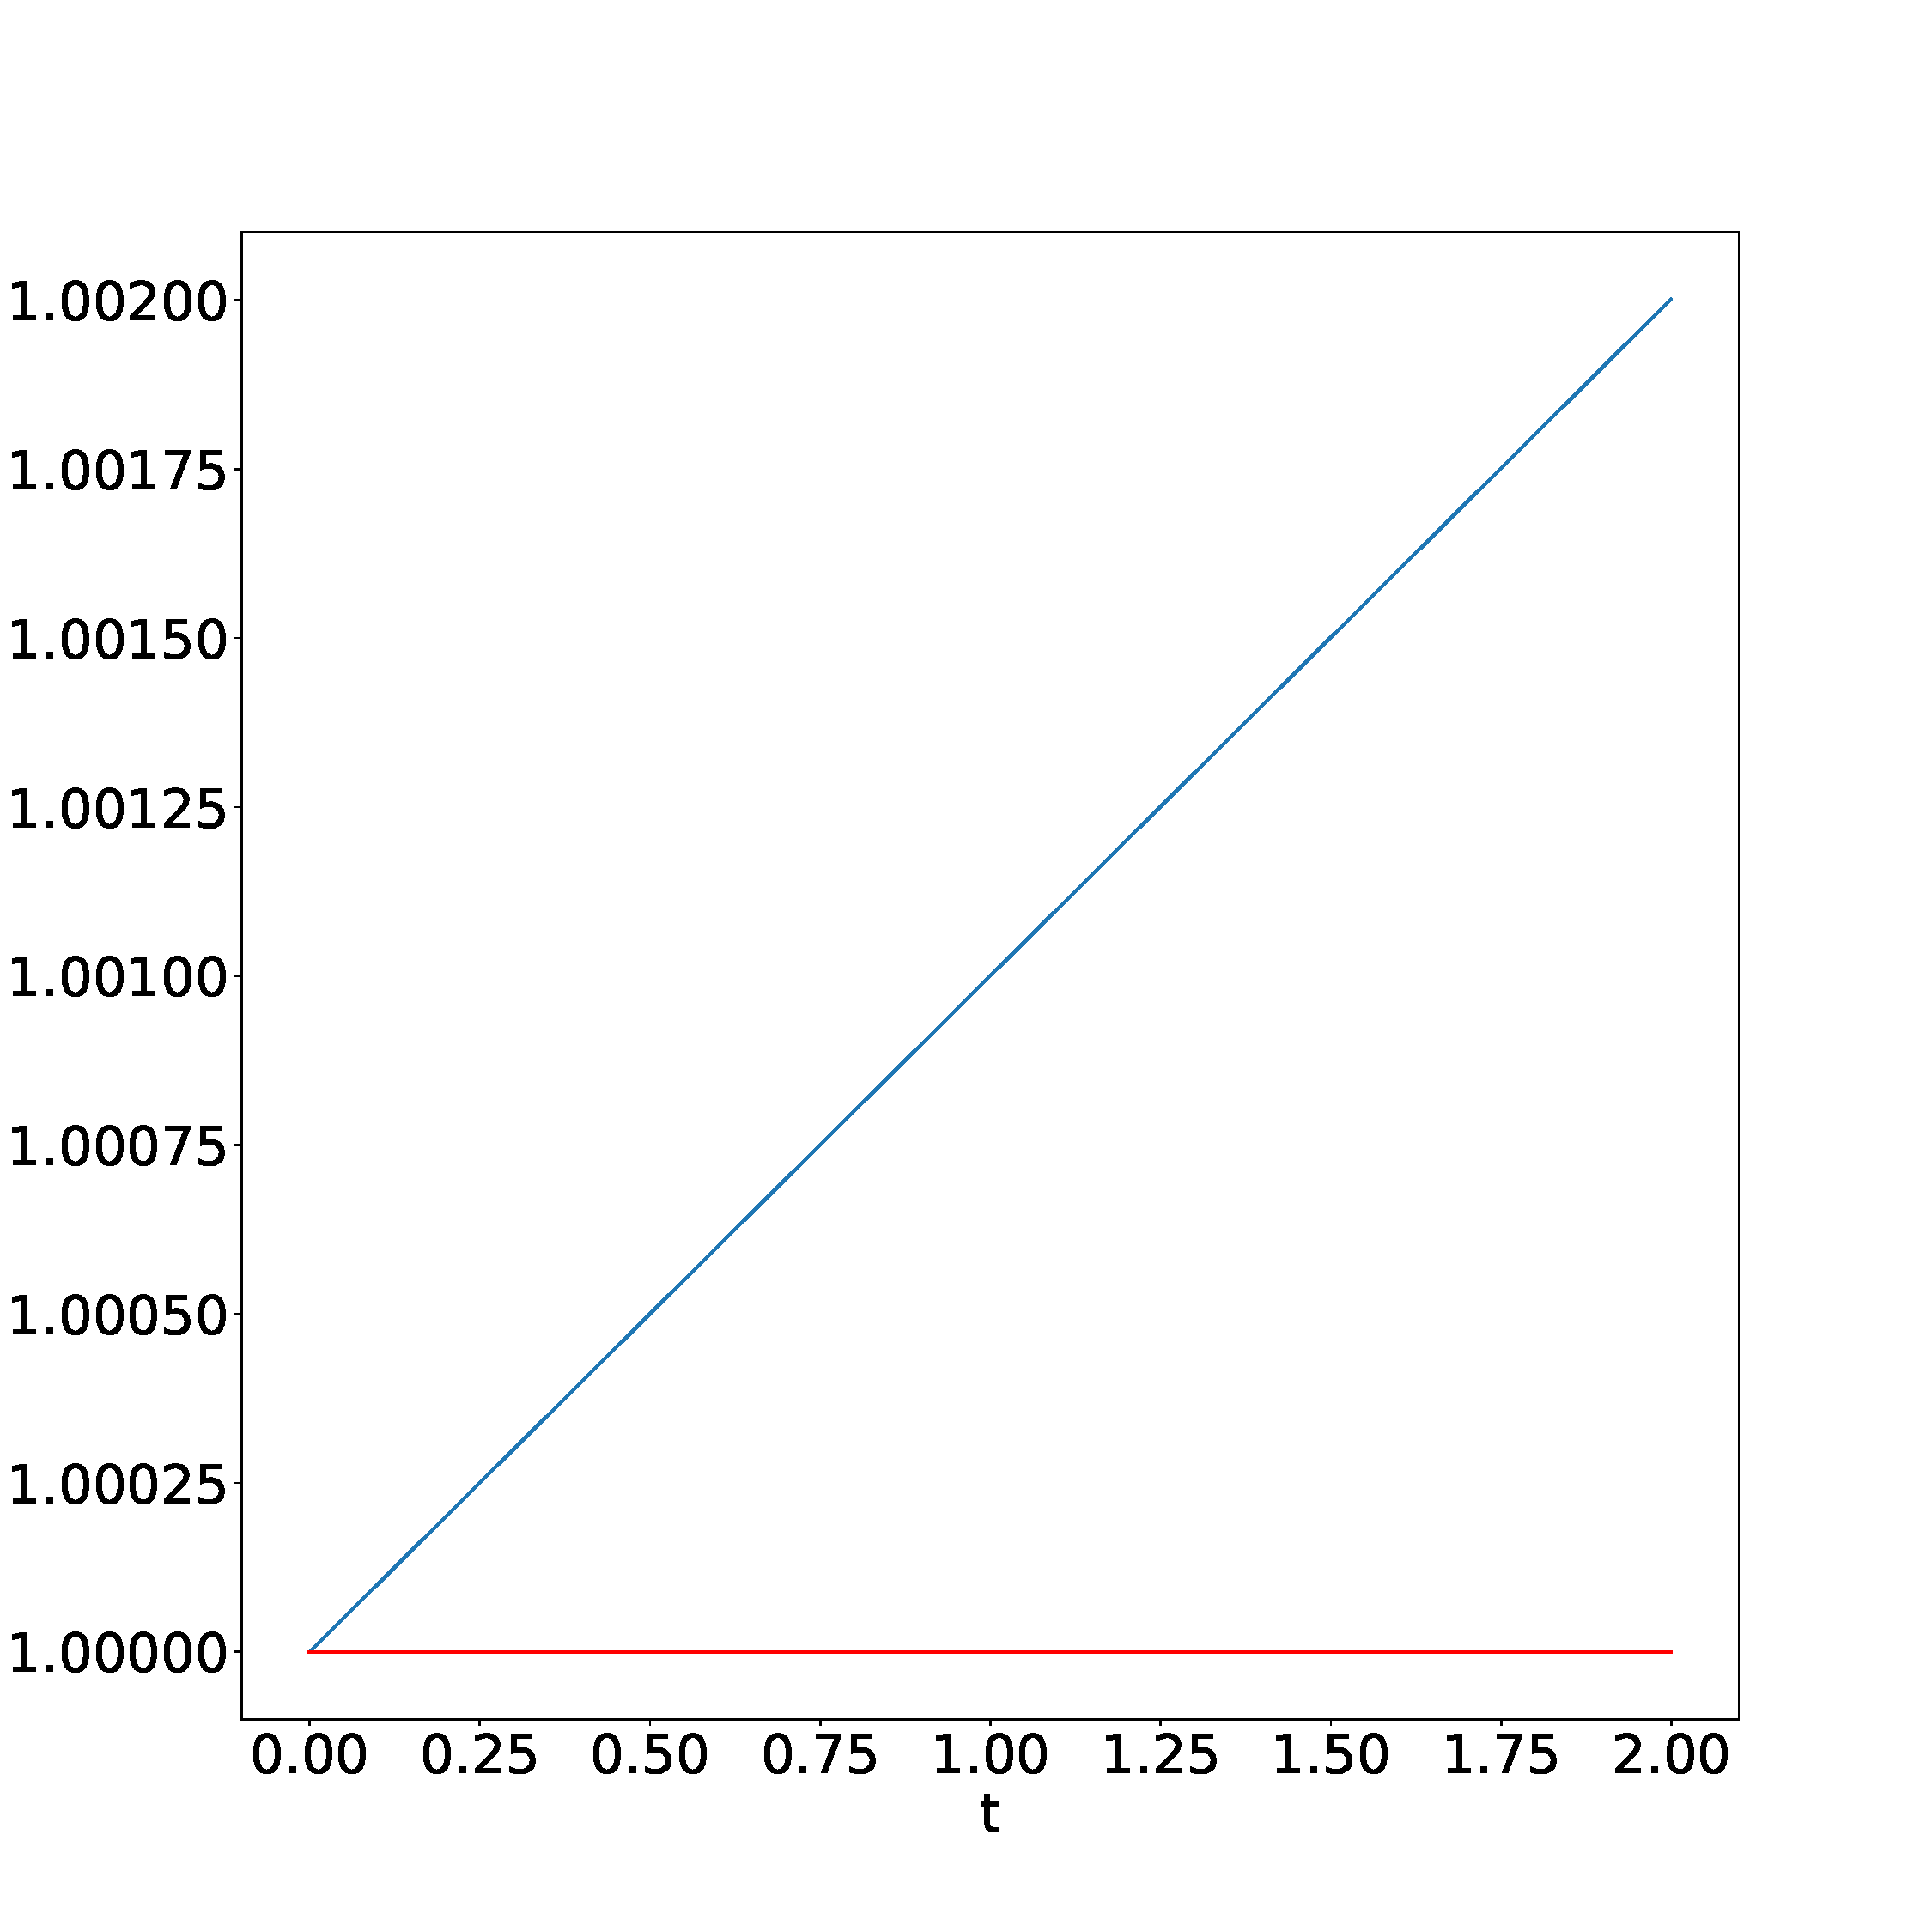
\includegraphics[width=.5\textwidth, height=.35\textheight]{energyPlot.pdf}
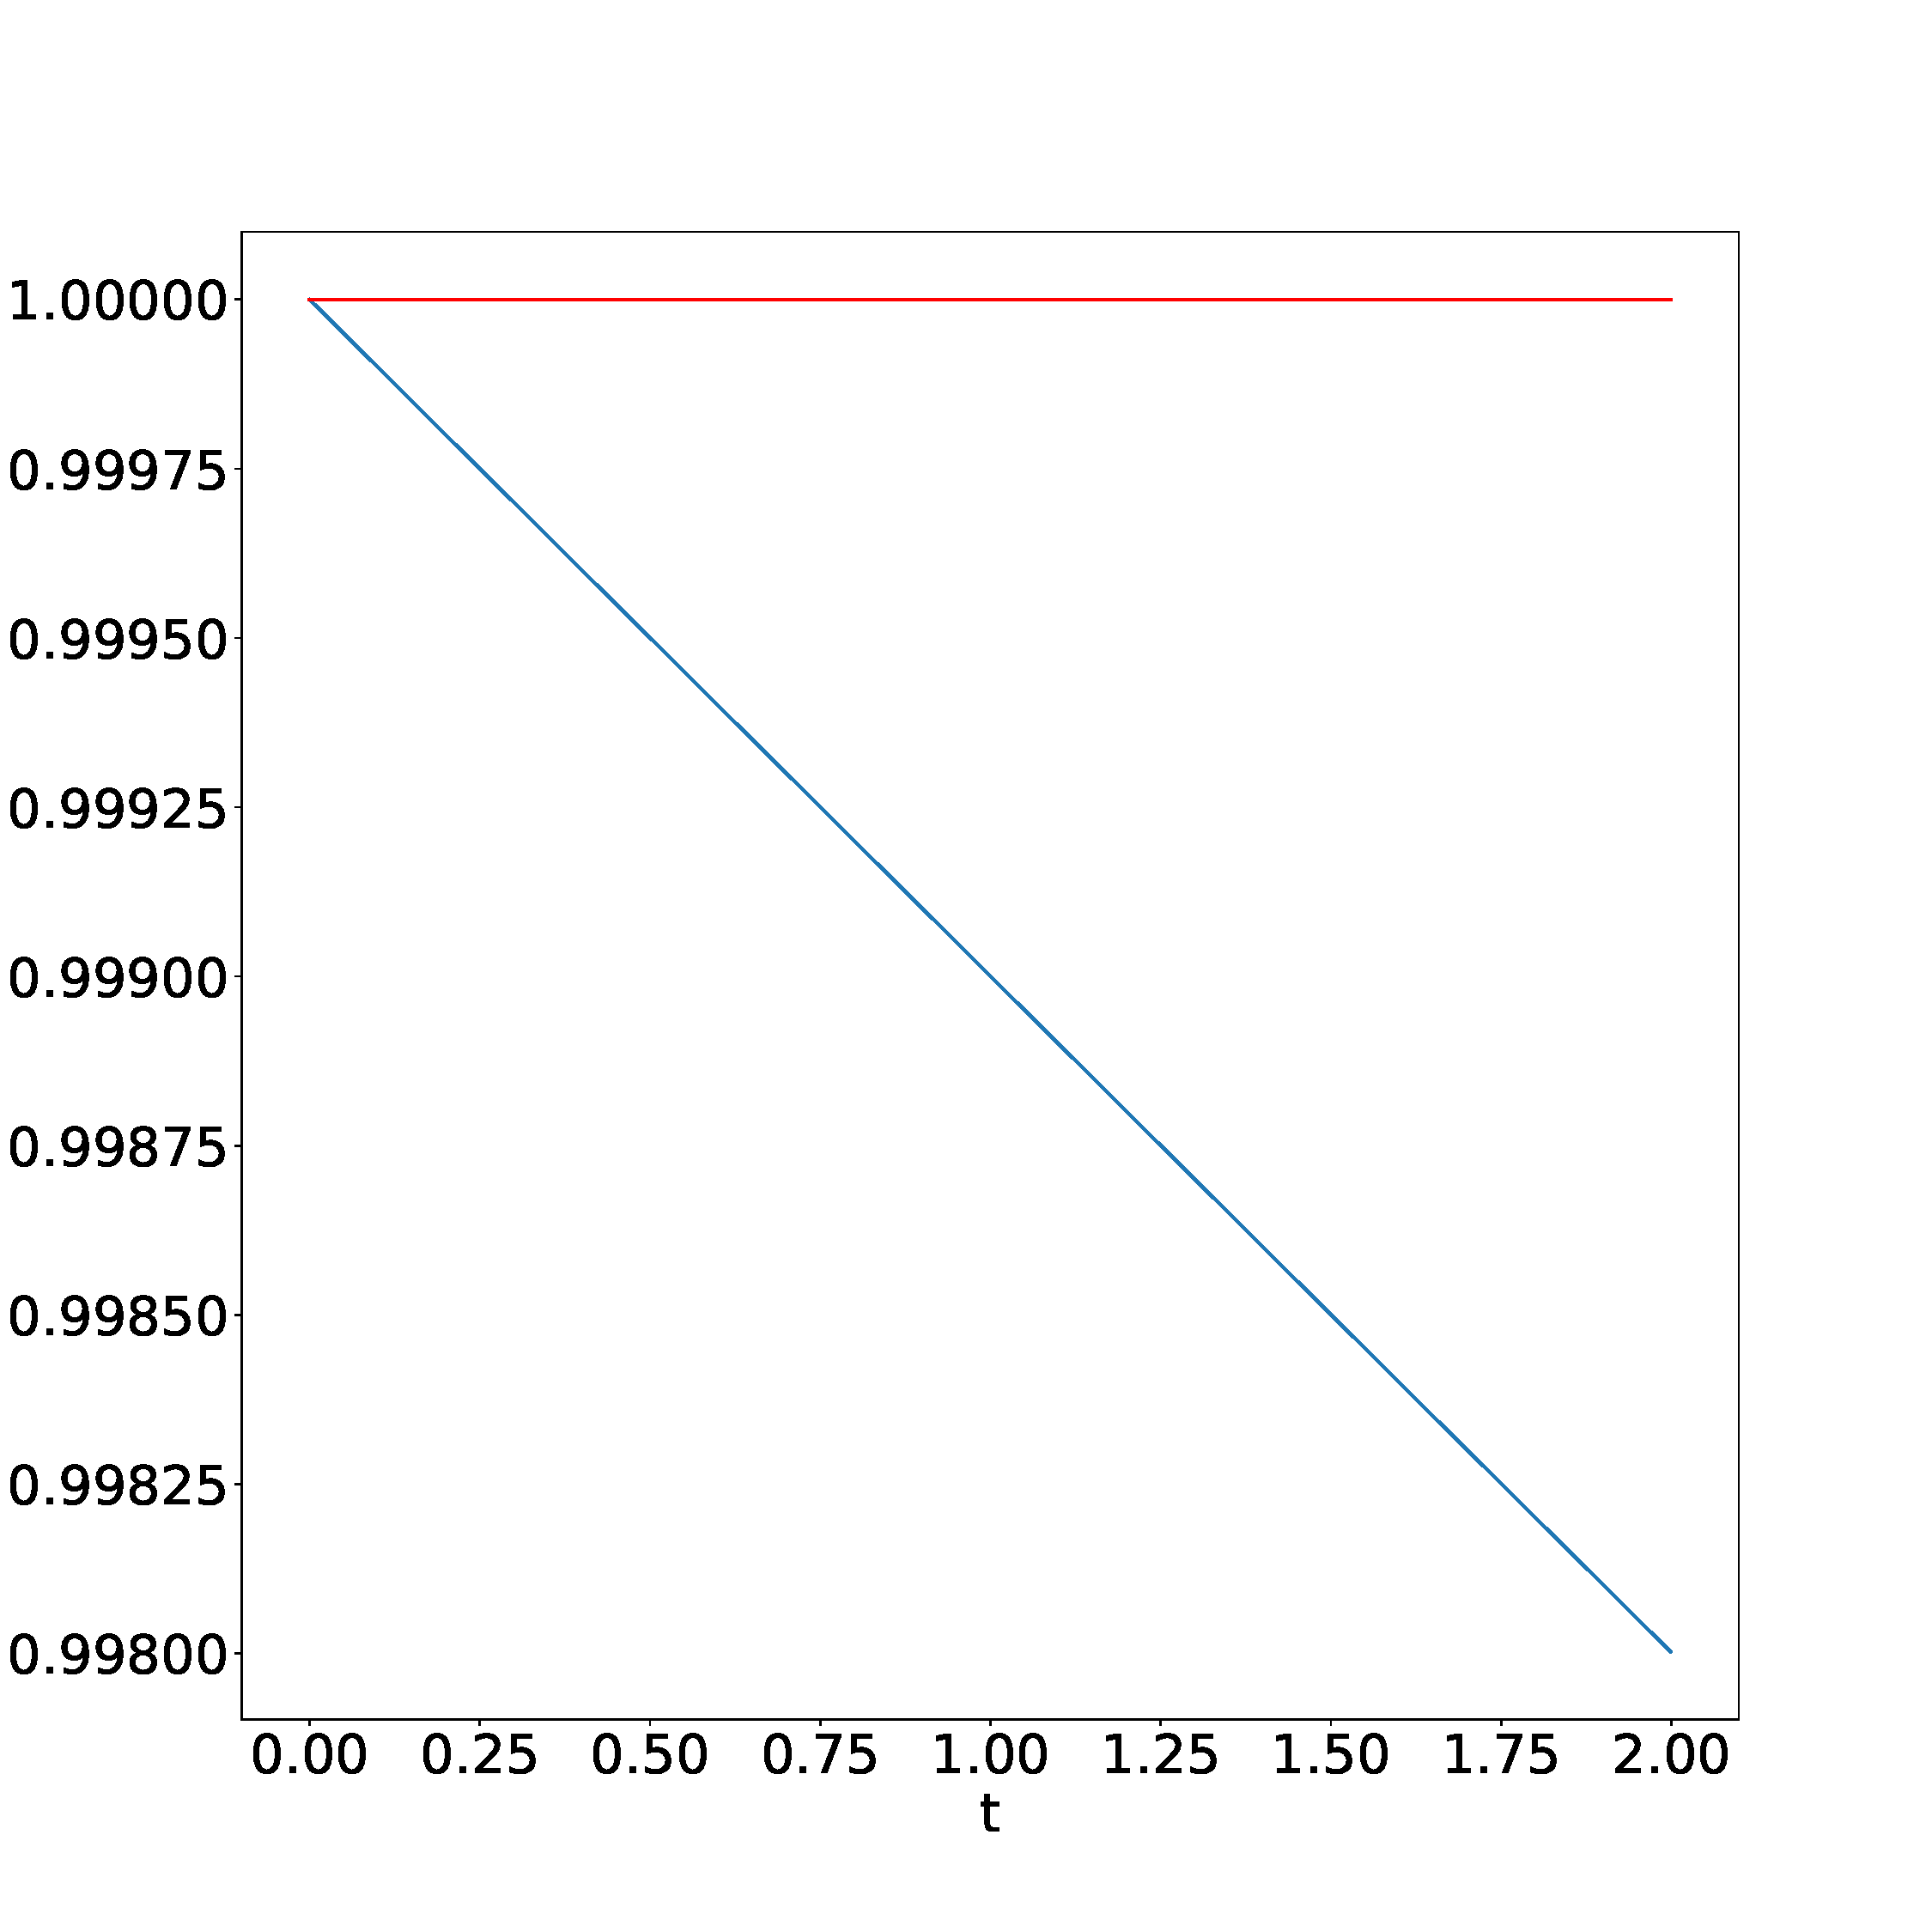
\includegraphics[width=.5\textwidth, height=.35\textheight]{energy2.pdf}
\caption{Energy as a function of time for both the explicit (left) and implicit (right) Euler methods, where the blue lines represent the Euler method energy and the red line represents the exact energy. The explicit method overestimates the total energy of the system, while the implicit method underestimates the energy. Both plots show a linear long-term trend for the energy errors, which makes sense given that the global error plots appear to be bounded by a linear function (although they oscillate sinusoidally). Both plots are made with $x(0) = 1$, $v(0) = 0$, $t(0) = 0$, and $h = .001$.}
\end{figure}

\begin{figure}[H]
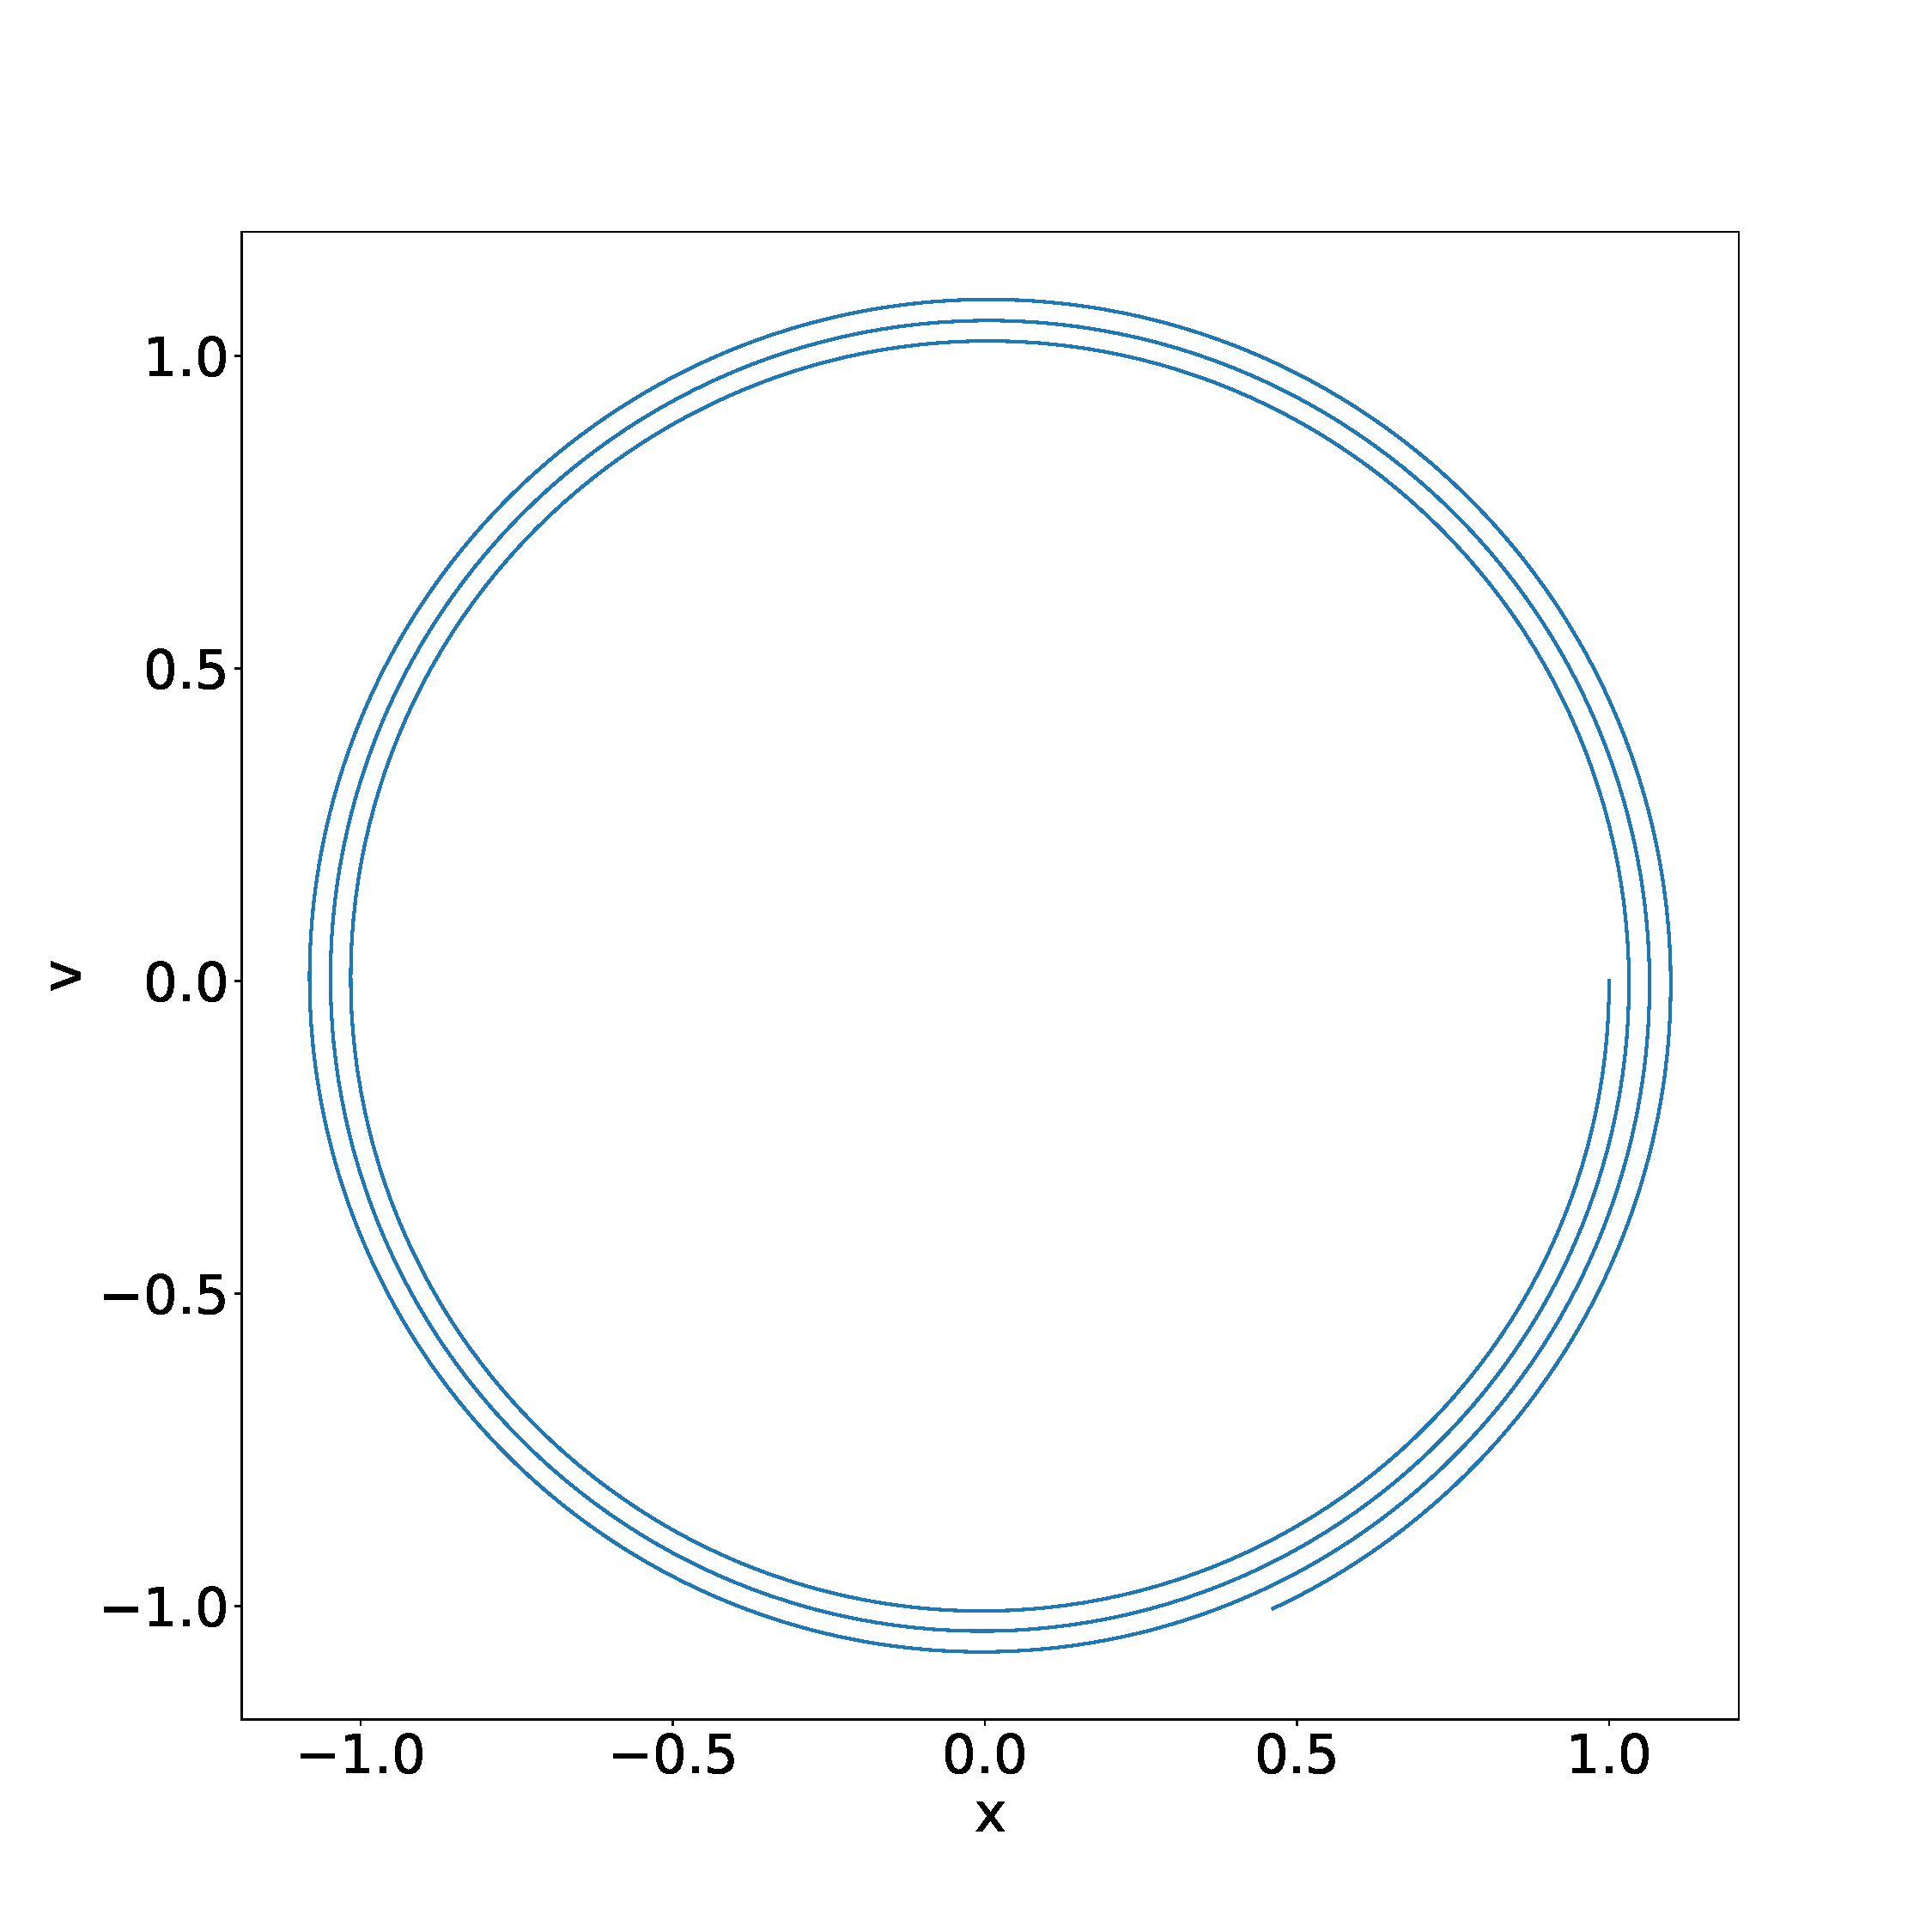
\includegraphics[width=.5\textwidth, height=.35\textheight]{XvsVexplicit.pdf}
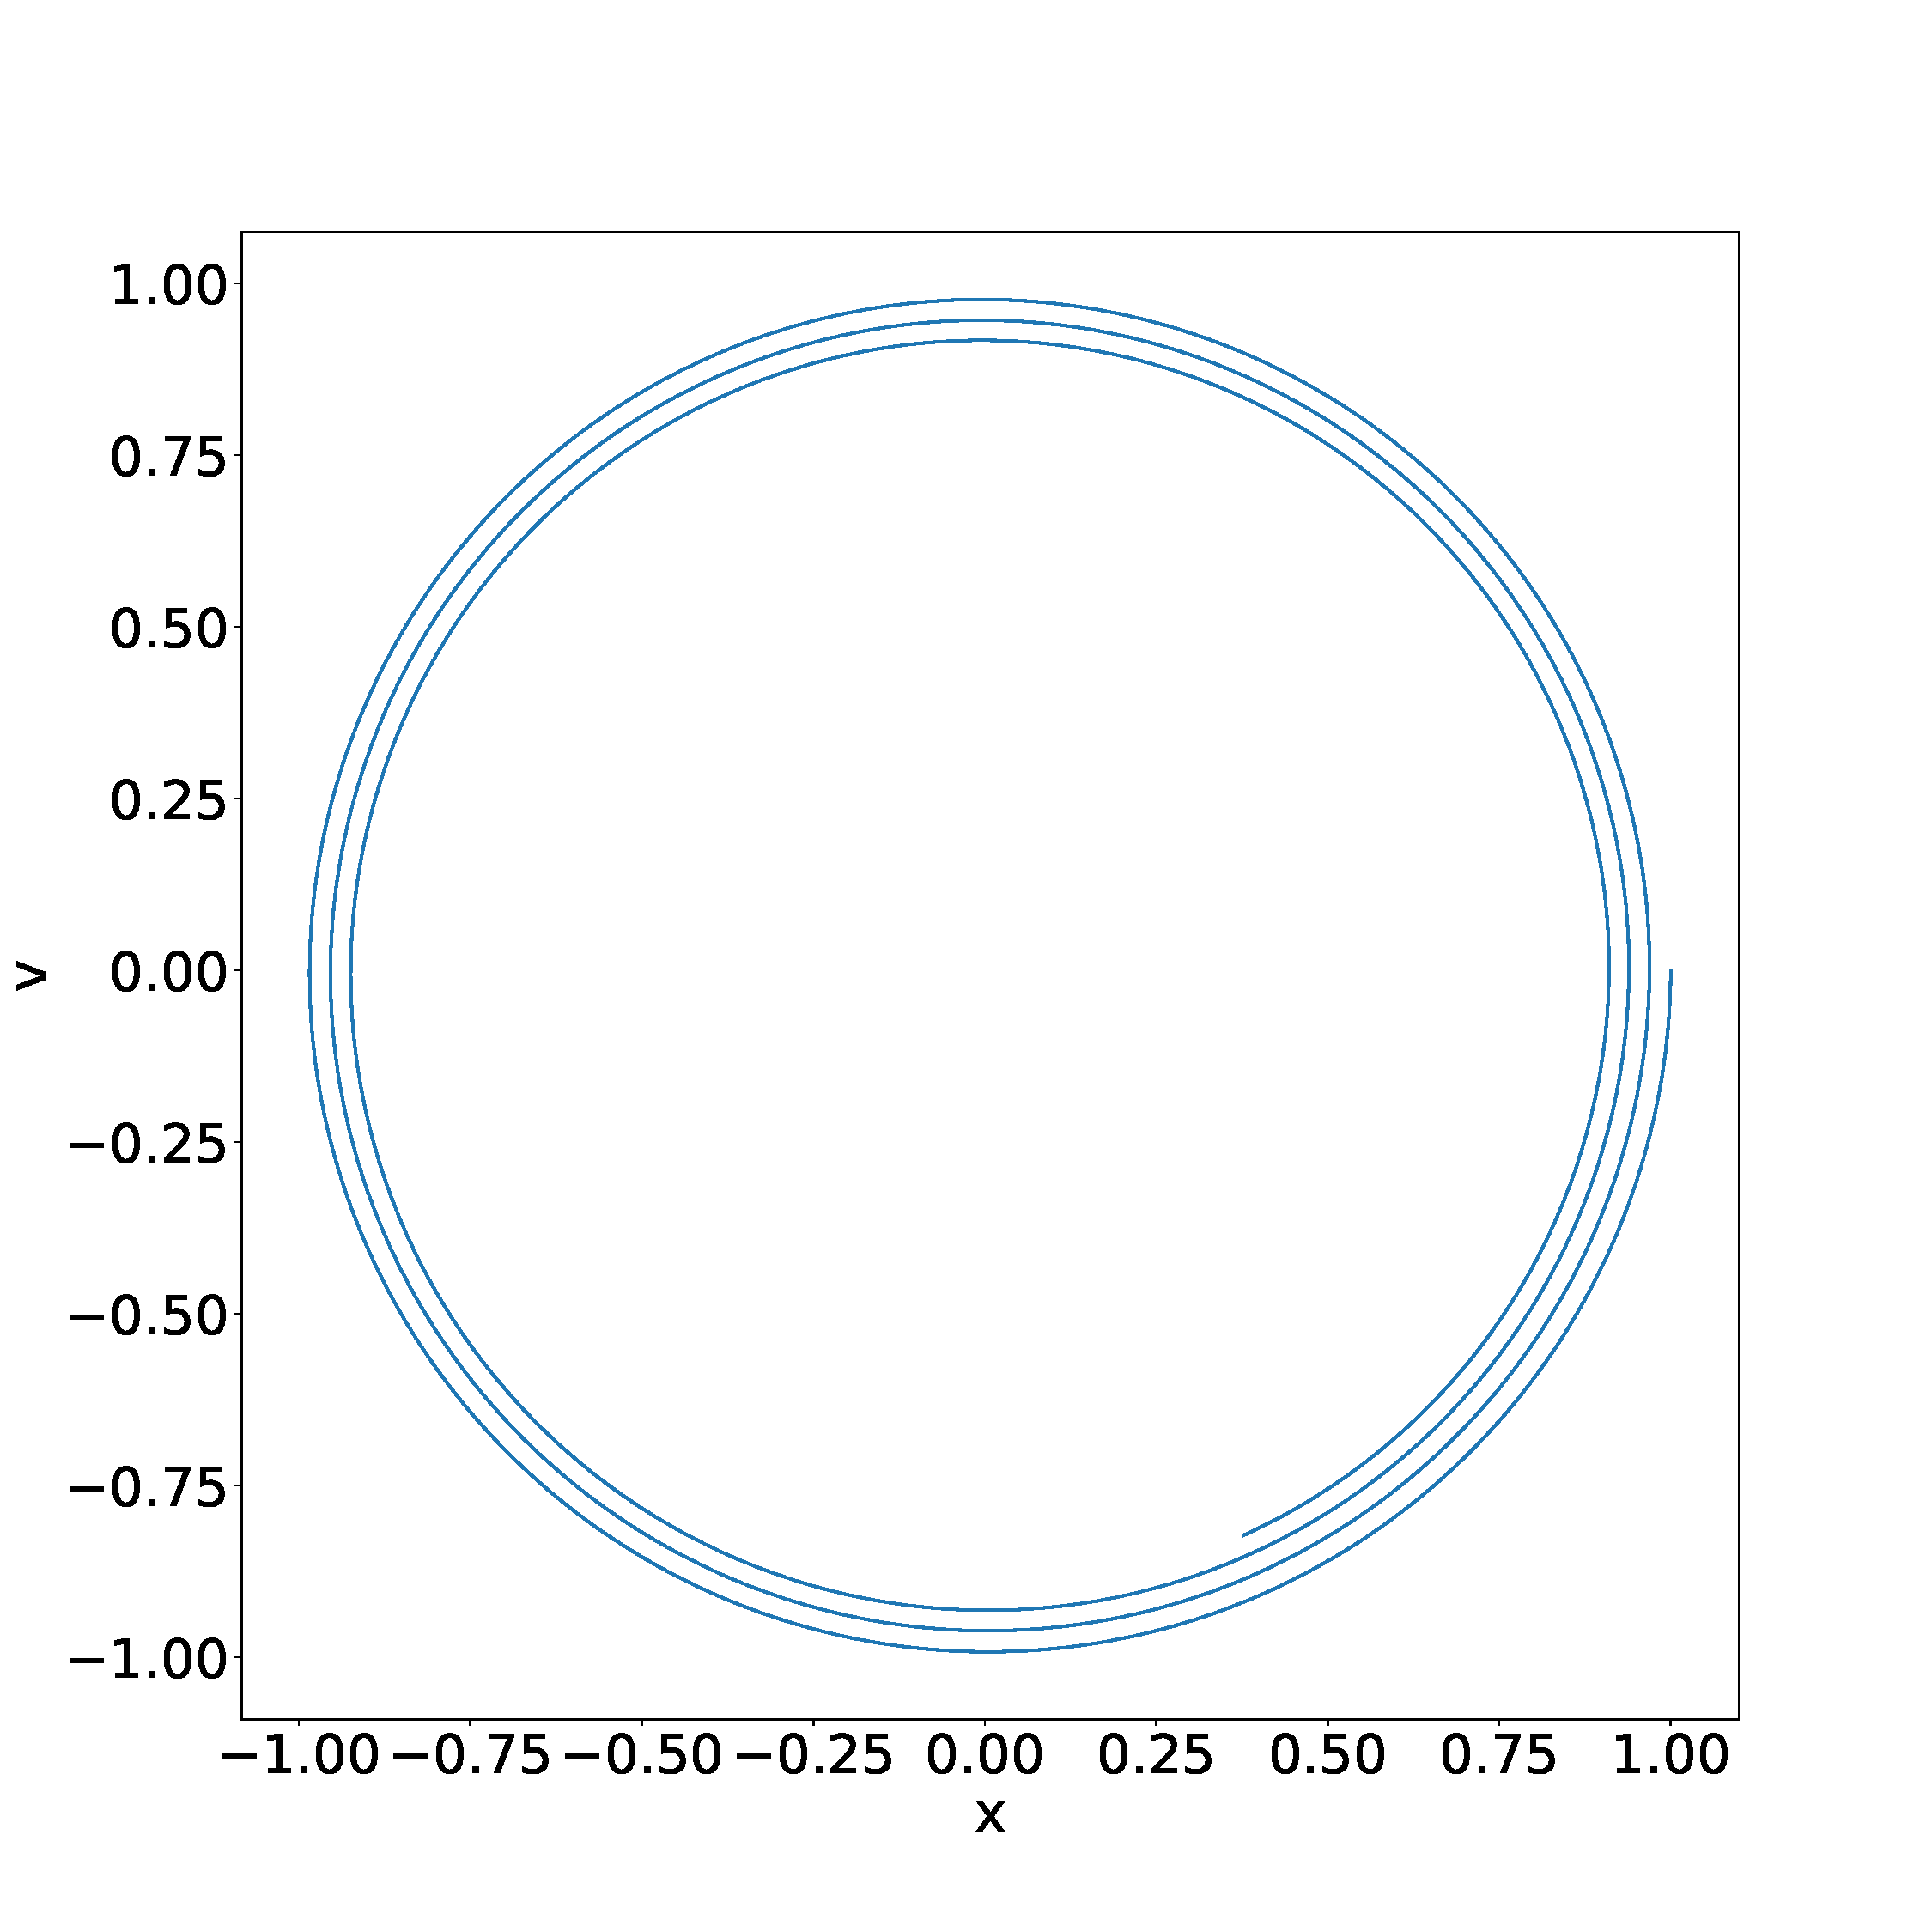
\includegraphics[width=.5\textwidth, height=.35\textheight]{XvsVimplicit.pdf}
\caption{Phase space plot of $x$ vs. $v$ for the explicit (left) and implicit (right) Euler methods. Both plots spiral clockwise, with the explicit plot growing outwards with time and the implicit plot growing inwards with time. This is consistent with the energy $E = x^2 + v^2$ of the explicit plot, increasing with time, and the energy of the implicit plot decreasing with time. Both plots are made with $x(0) = 1$, $v(0) = 0$, $t(0) = 0$, and $h = .001$.}
\end{figure}

\begin{figure}[H]
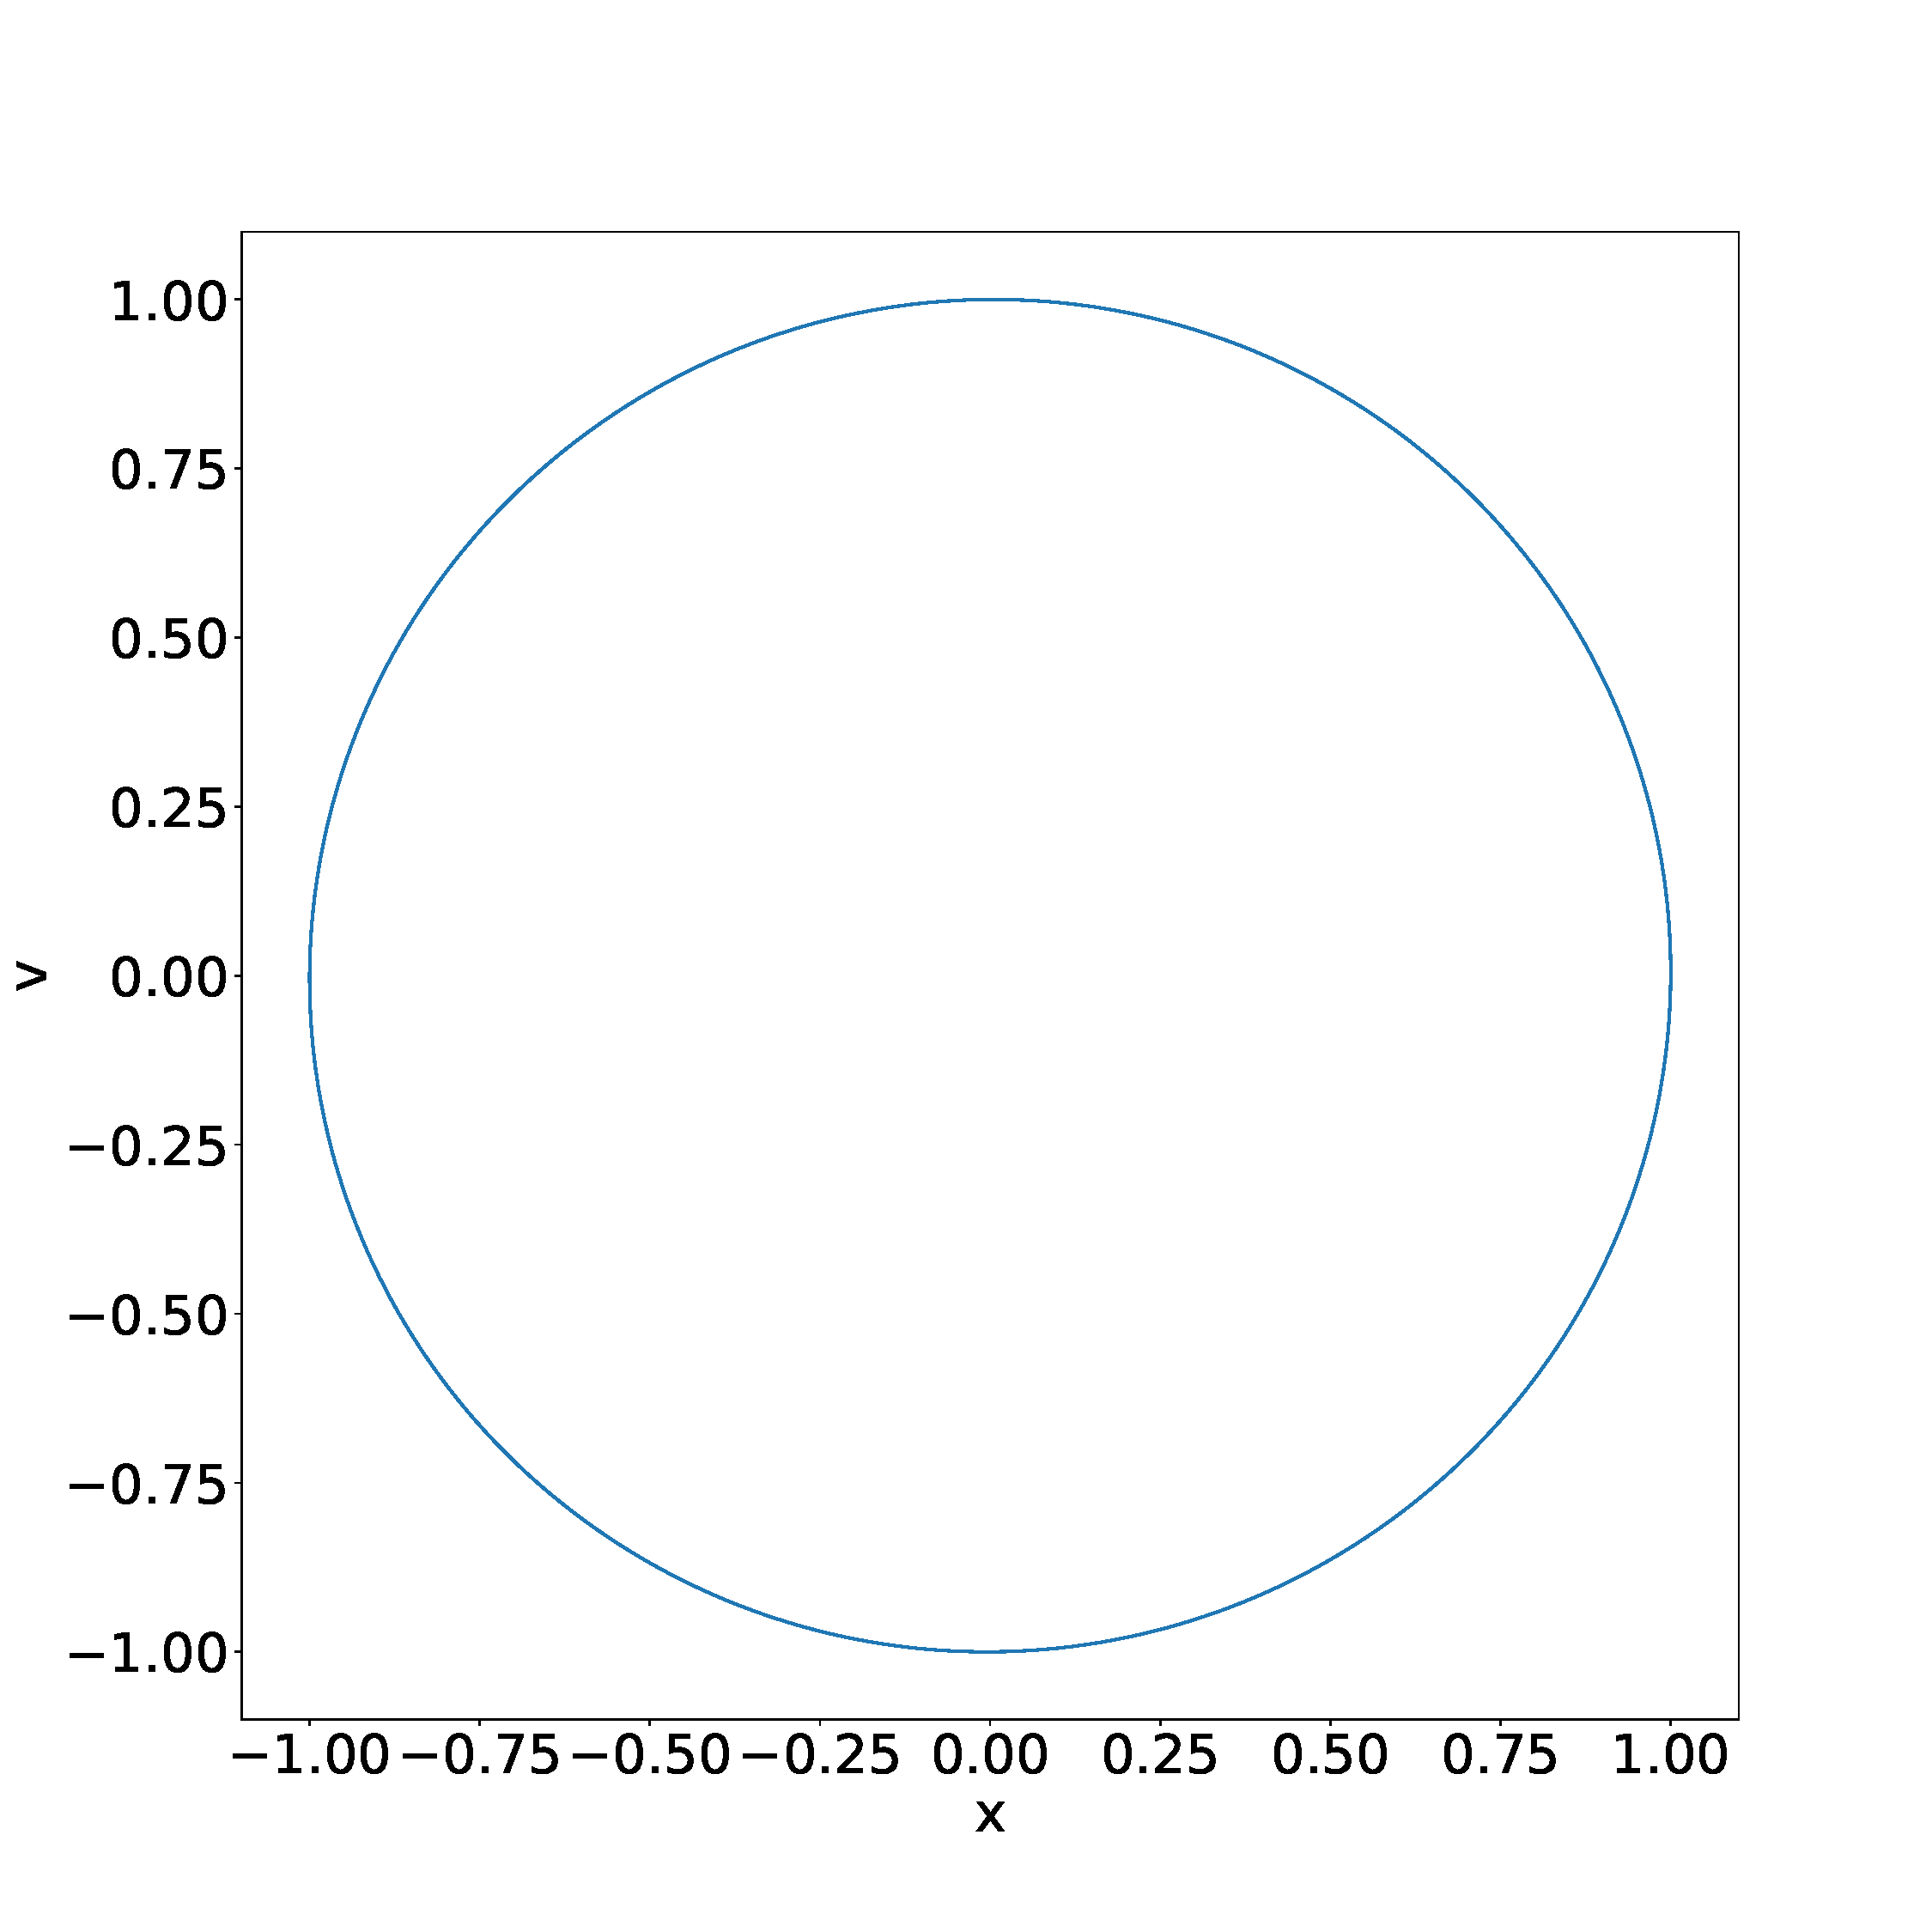
\includegraphics[width=.5\textwidth, height=.35\textheight]{XvsVsymp.pdf}
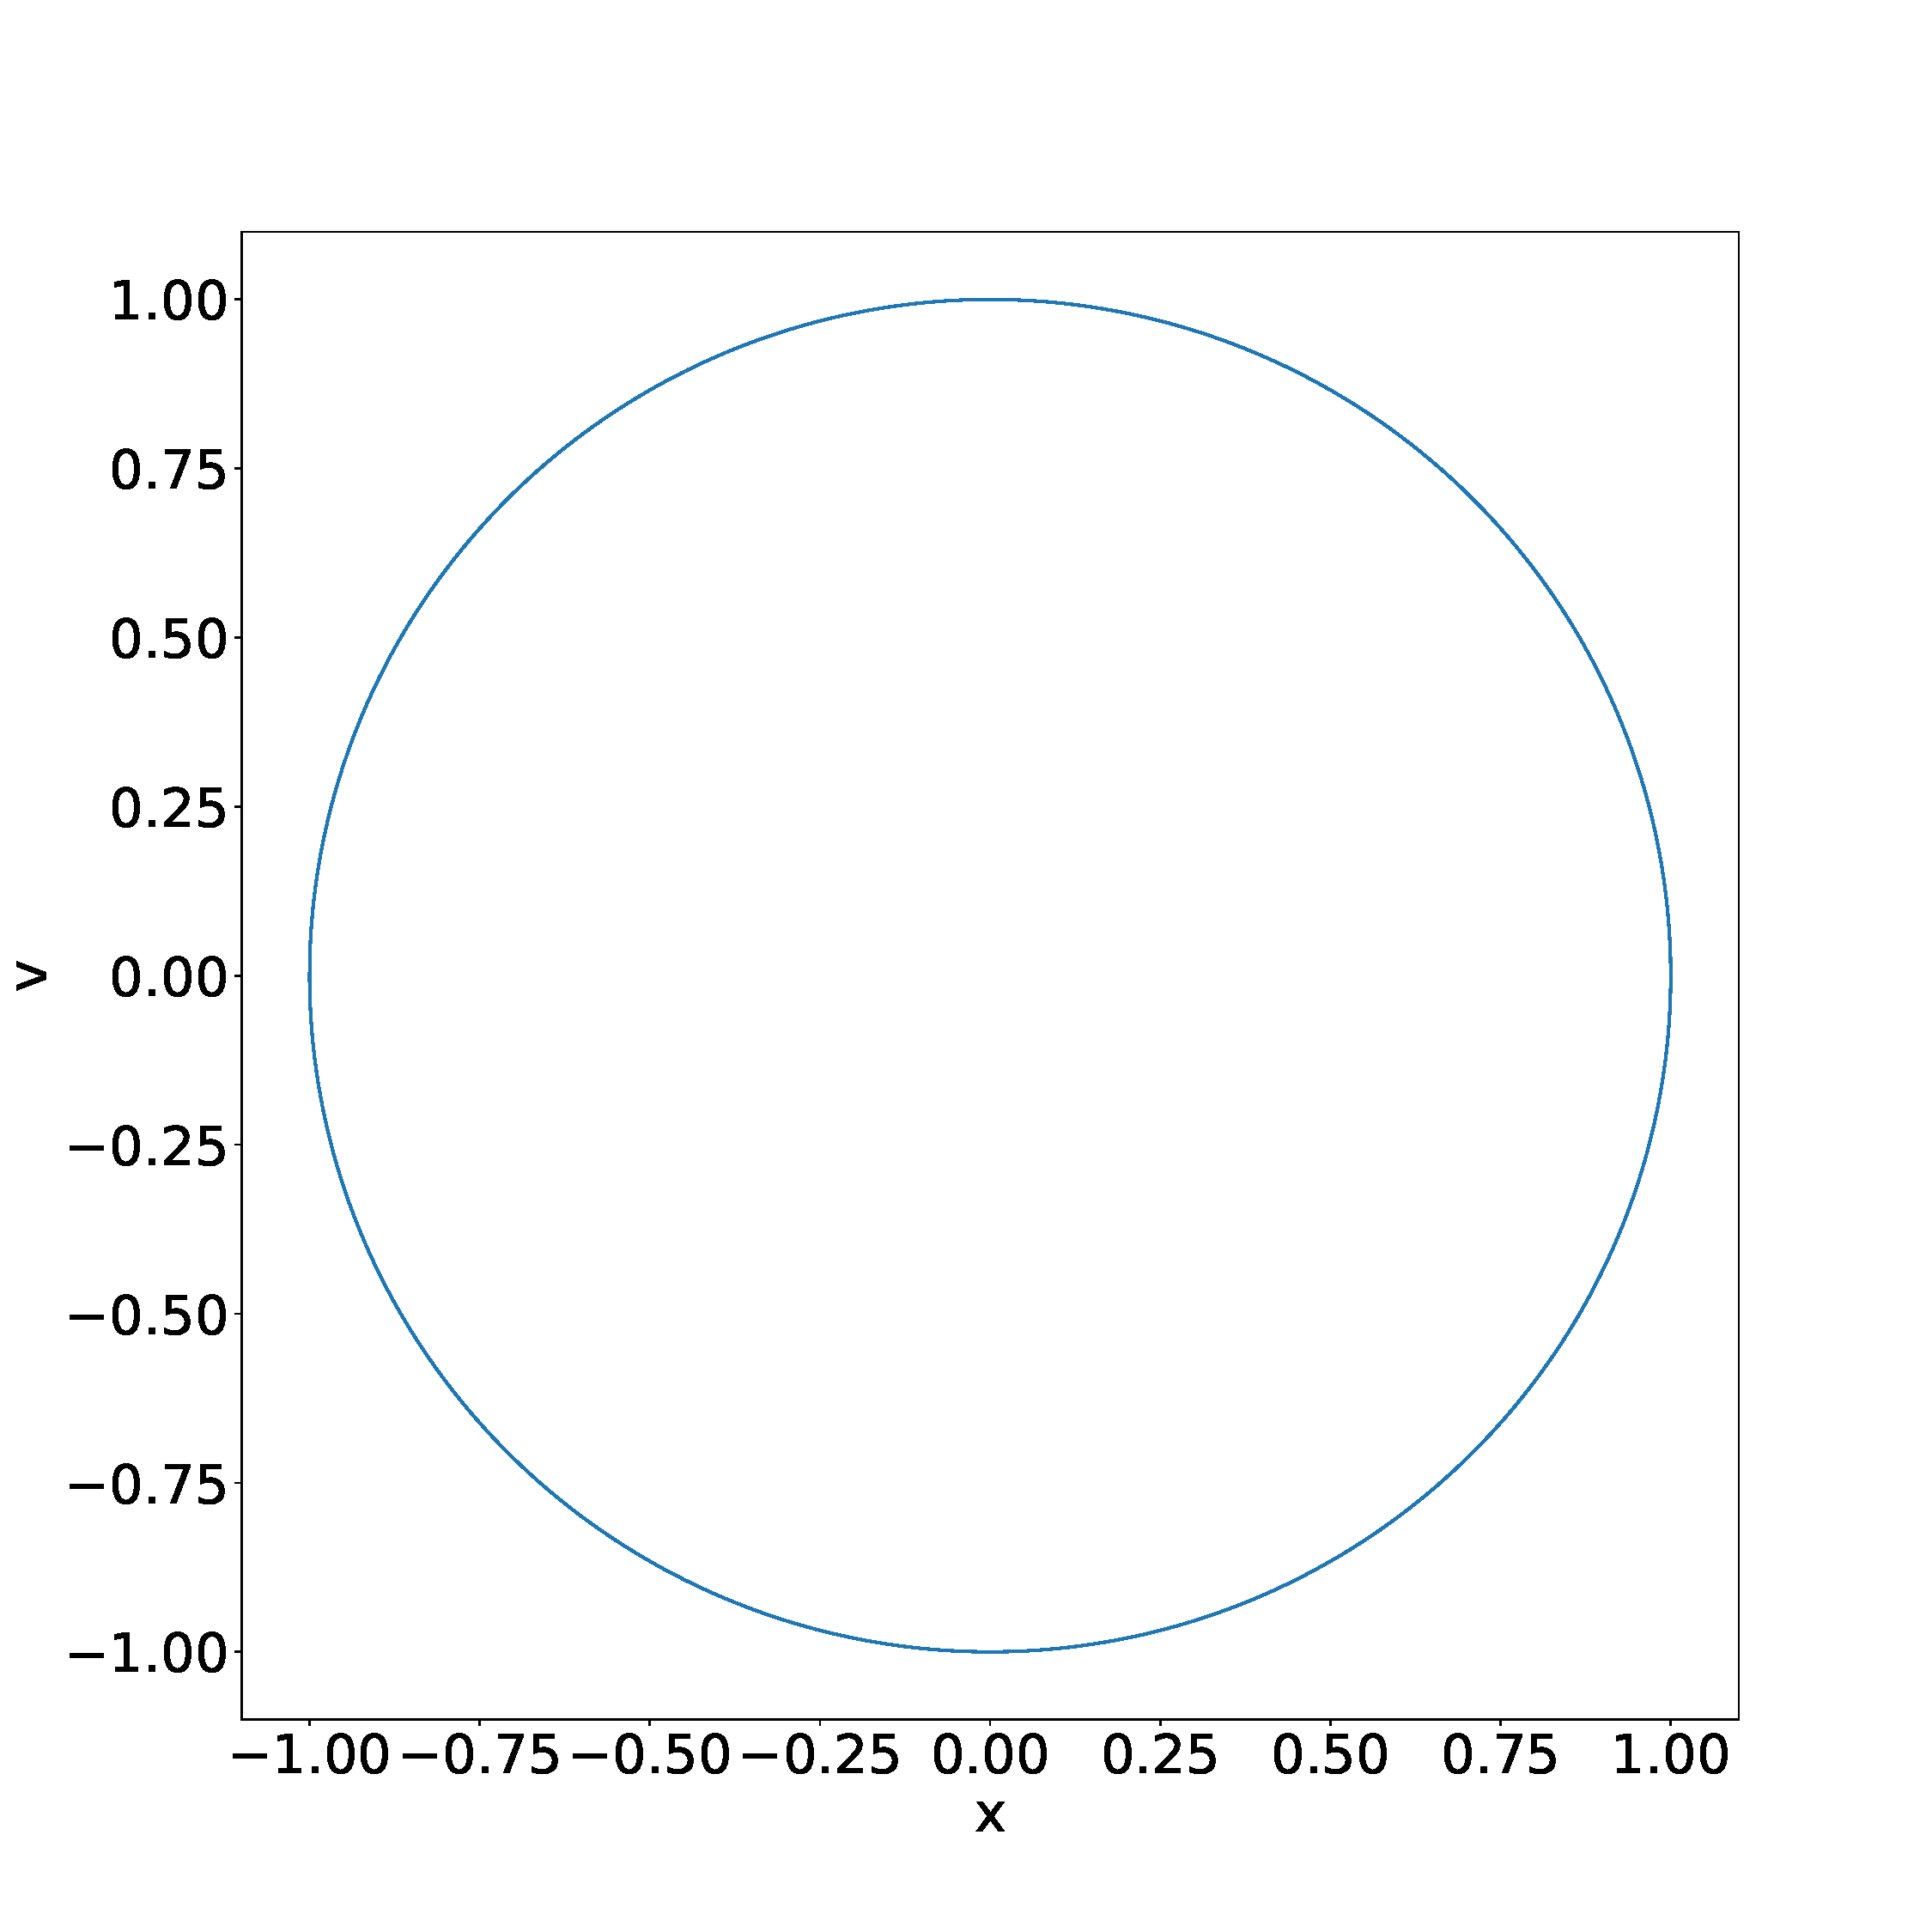
\includegraphics[width=.5\textwidth, height=.35\textheight]{XvsVtrue.pdf}
\caption{Phase space plot of $x$ vs. $v$ for the symplectic (left) Euler method, compared to the phase space plot for the exact solution (right). While there are errors in the symplectic method, the errors oscillate sinusoidally (see figure 7), so they average out and the phase space curves appear to match. Both plots are made with $x(0) = 1$, $v(0) = 0$, $t(0) = 0$, and $h = .001$.}
\end{figure}

\begin{figure}[H]
\centerline{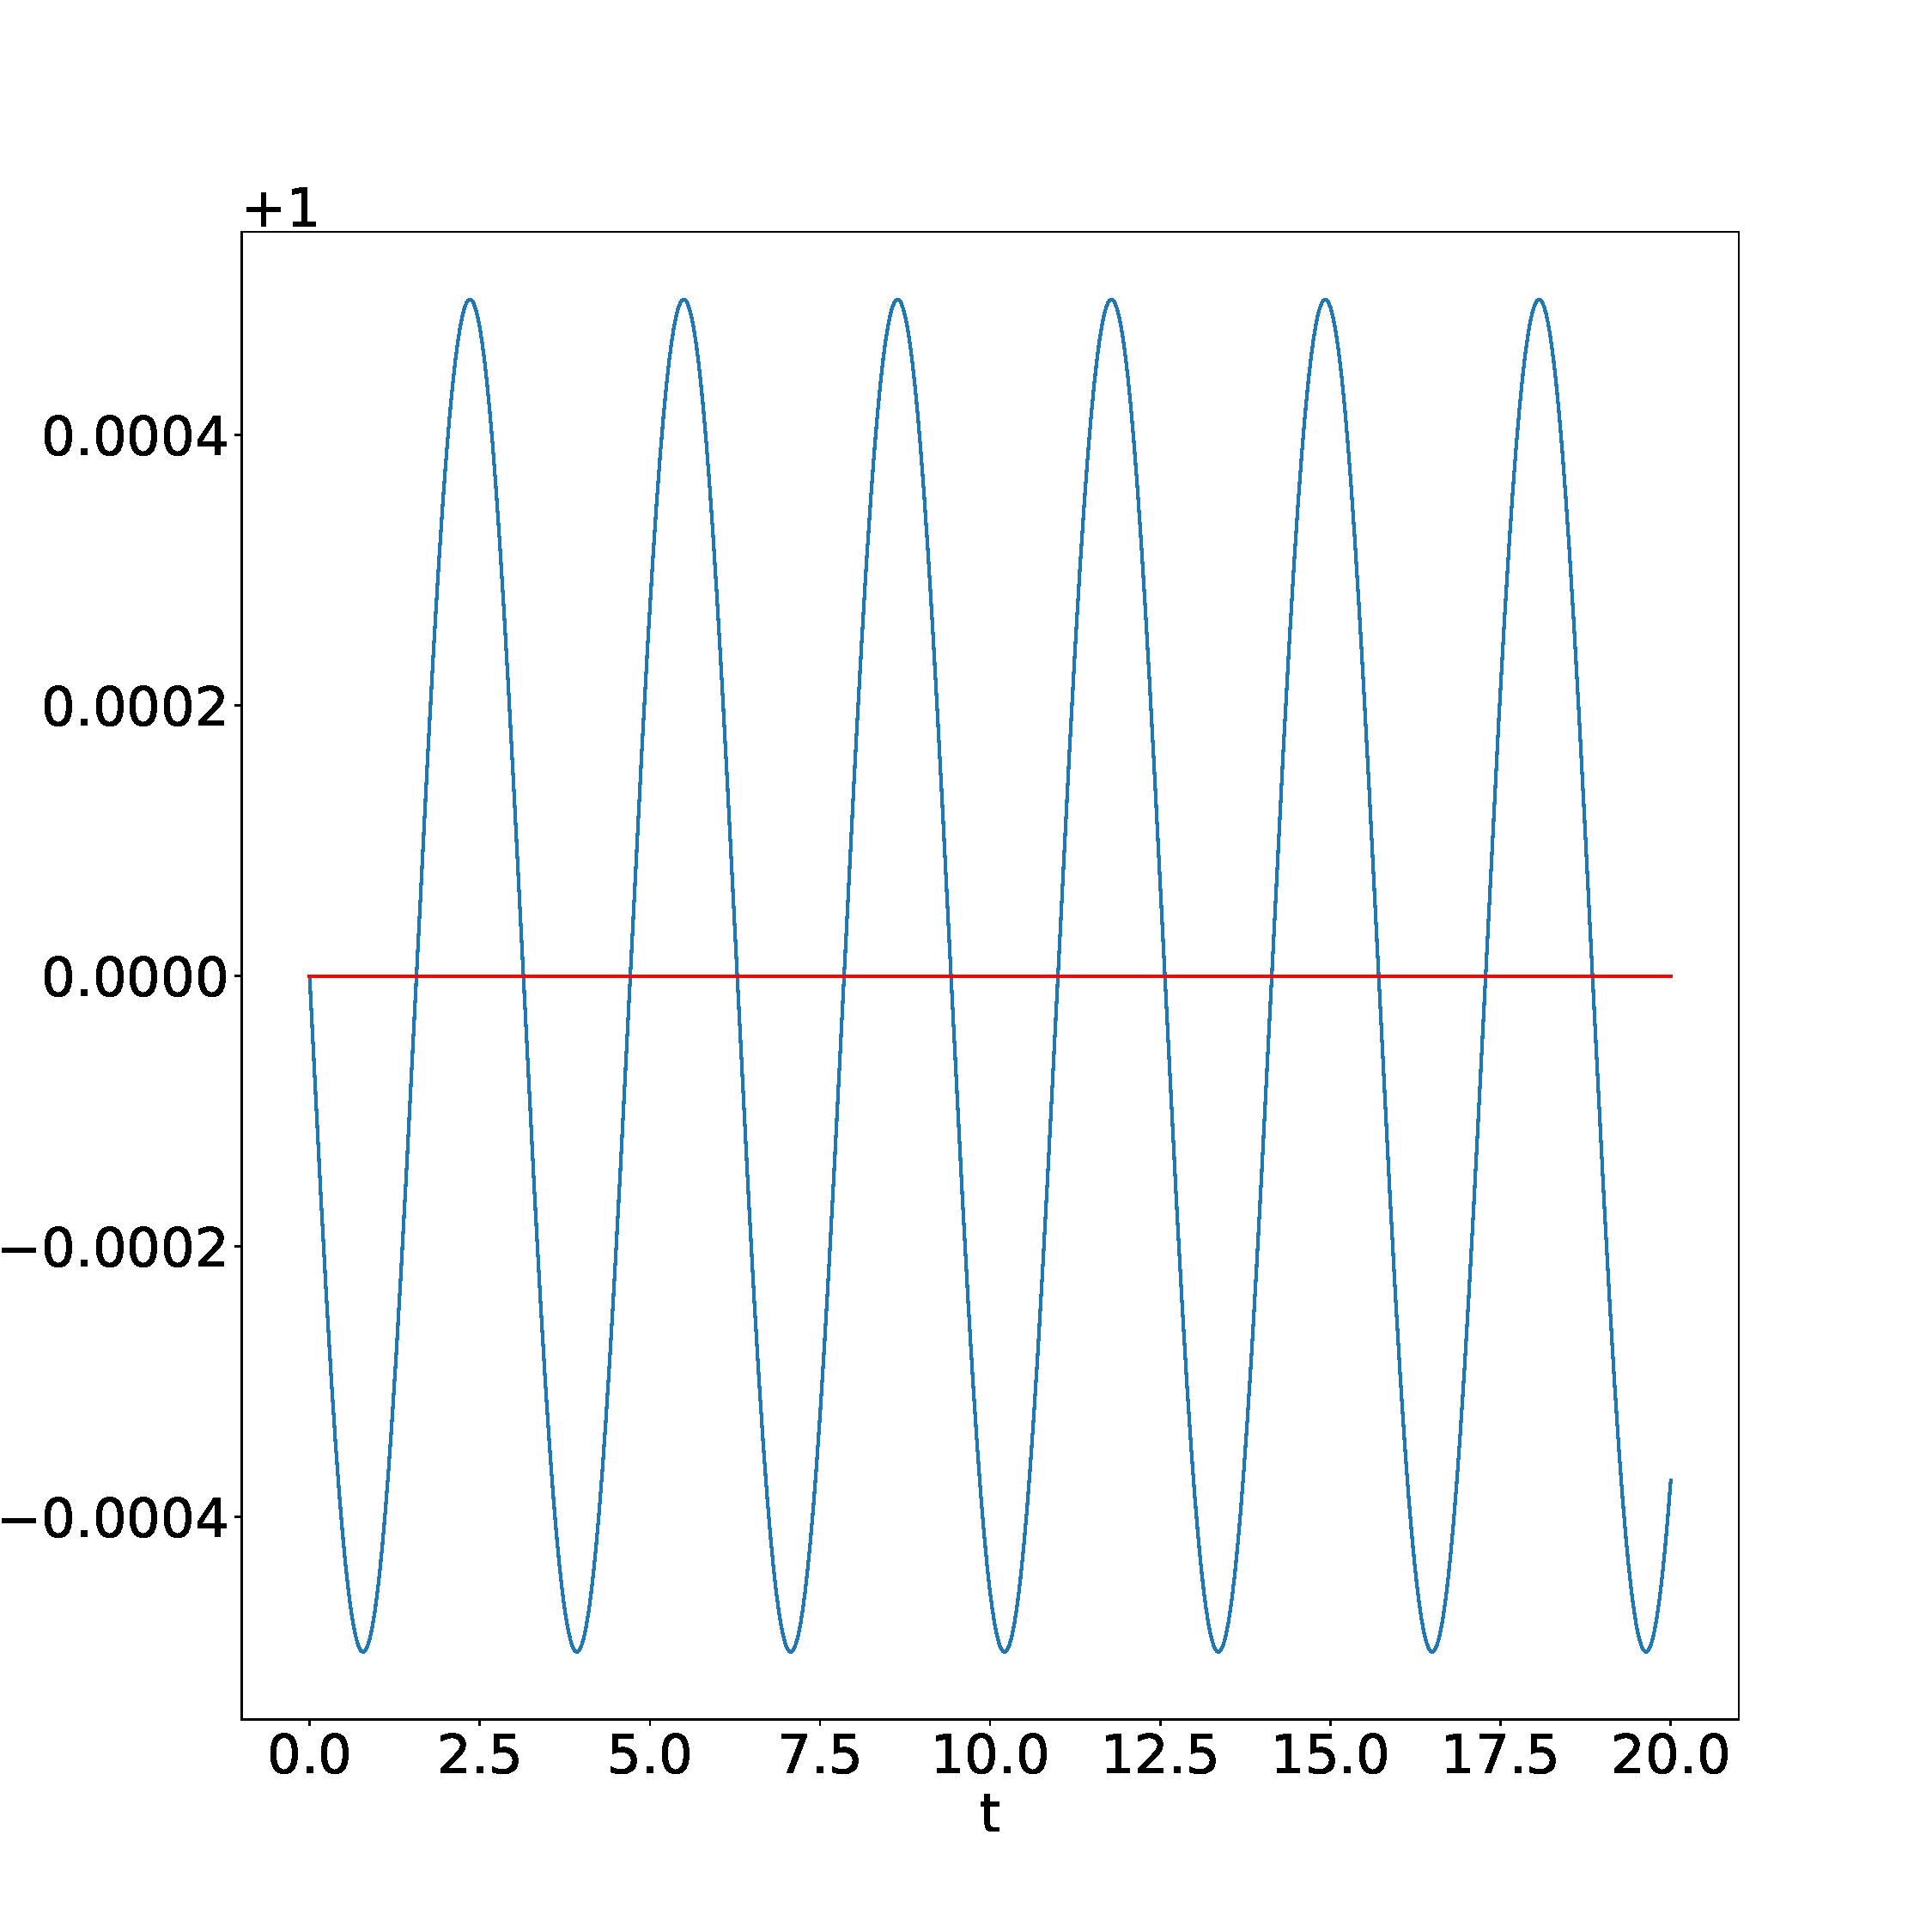
\includegraphics[width=.7\textwidth, height=.5\textheight]{sympError.pdf}}
\caption{Energy as a function of time for both the symplectic Euler method (left), and the exact solution (right, energy remains constant). The difference between the two energies oscillates sinusoidally as time goes on, leading to phase space plots that look identical. Both energy plots are made with $x(0) = 1$, $v(0) = 0$, $t(0) = 0$, and $h = .001$.}
\end{figure}

\end{section}

\end{document}  